%%%%%%%%%%%%%%%%%%%%%%%%%%%%%%%%%%%%%%%%%%%%%%%%%%%%%%%%%%%%%%%%%
%_____________ ___    _____  __      __ 
%\____    /   |   \  /  _  \/  \    /  \  Institute of Applied
%  /     /    ~    \/  /_\  \   \/\/   /  Psychology
% /     /\    Y    /    |    \        /   Zürcher Hochschule 
%/_______ \___|_  /\____|__  /\__/\  /    fuer Angewandte Wissen.
%        \/     \/         \/      \/                           
%%%%%%%%%%%%%%%%%%%%%%%%%%%%%%%%%%%%%%%%%%%%%%%%%%%%%%%%%%%%%%%%%
%
% Project     : Seminararbeit
% Title       : 
% File        : doc.tex Rev. 00
% Date        : 10.10.2012
% Author      : Till J. Ernst
%
%%%%%%%%%%%%%%%%%%%%%%%%%%%%%%%%%%%%%%%%%%%%%%%%%%%%%%%%%%%%%%%%%

%%%%%%%%%%%%%%%%%%%%%%%%%%%%%%%%%%%%%%%%%%%%%%%%%%%%%%%%%%%%%%%%%
%  _____   ____  _____                                          %
% |_   _| /  __||  __ \    Institute of Computitional Physics   %
%   | |  |  /   | |__) |   Zuercher Hochschule Winterthur       %
%   | |  | (    |  ___/    (University of Applied Sciences)     %
%  _| |_ |  \__ | |        8401 Winterthur, Switzerland         %
% |_____| \____||_|                                             %
%%%%%%%%%%%%%%%%%%%%%%%%%%%%%%%%%%%%%%%%%%%%%%%%%%%%%%%%%%%%%%%%%
%
% Project     : LaTeX doc Vorlage für Windows ProTeXt mit TexMakerX
% Title       : 
% File        : header.tex Rev. 00
% Date        : 23.4.12
% Author      : Remo Ritzmann
% Feedback bitte an Email: remo.ritzmann@pfunzle.ch
%
%%%%%%%%%%%%%%%%%%%%%%%%%%%%%%%%%%%%%%%%%%%%%%%%%%%%%%%%%%%%%%%%%

\documentclass[
	oneside,
	10pt,
	parskip=half,
	ngerman,
	%bibtotocnumbered,
	%bibliography=totocnumbered,
	listof=totoc,
	version=first
	%liststotoc
]{scrreprt}
%article scrartcl
%report scrreprt
%book scrbook
%letter scrlttr2

%***********************************************************************
% include some libs
%***********************************************************************	
\usepackage[utf8]{inputenc}
\usepackage{listings}
\usepackage{color}
\usepackage{fancyhdr}
\usepackage{rotating}
\usepackage{titlesec}
\usepackage{mathptmx} 
\usepackage[scaled=.90]{helvet}
%\usepackage{times}
%\renewcommand*\familydefault{\sfdefault} %% Only if the base font of the document is to be sans serif
\usepackage[T1]{fontenc}
\usepackage{german}
%\usepackage[ngerman]{babel}
%\usepackage[babel]{csquotes}
\usepackage{textcomp}
\usepackage[squaren]{SIunits}
\usepackage{graphicx}
\usepackage{url}
\usepackage{geometry}
\usepackage[absolute]{textpos}
\usepackage{makeidx}
\usepackage{colortbl}
\usepackage{pdflscape}
\usepackage{pdfpages}
\usepackage{tabularx}
\usepackage{lmodern}
\usepackage{longtable}
\usepackage{array}
\usepackage{float}
\usepackage{scrhack}
\usepackage{wallpaper}
\usepackage{titleref}

% Bereitstellung Hyperlinkfunktionen (PDF) (muss als letztes Paket geladen werden)
\usepackage[
	colorlinks=true,
	breaklinks=true,
	linkcolor=black,
	citecolor=black,
	urlcolor=black,
	anchorcolor=black,
	pdfpagelabels,
	pdftitle={Seminararbeit},
	pdfsubject={Facebook und der Glücksfaktor},
	pdfkeywords={KEYWORDS},
	pdfauthor={Till J. Ernst (ernsttil)}
]{hyperref}

\usepackage{apacite}

% biblatex-apa
%\usepackage[style=apa,
%			backend=biber,
%			babel=hyphen,
%			natbib=true
%			style=authoryear, 
%    		maxcitenames=2, 
%    		sorting=nyt,
%    		backref=true
%]{biblatex}
%\DeclareLanguageMapping{ngerman}{{ngerman-apa}} 
%\addbibresource{Literatur} %for biblatex


% Bereitstellung Glossar
\usepackage[toc]{glossaries}
\makeglossaries



%***********************************************************************
% various styles
%***********************************************************************	

%create index
\makeindex

%define pagestyle
\pagestyle{fancy}

%use sans-serif font 
%\renewcommand{\familydefault}{\sfdefault}

%define page margin
\geometry{a4paper, top=25mm, left=25mm, right=25mm, bottom=25mm,headsep=10mm,footskip=10mm}

%textpos parameter
\setlength{\TPHorizModule}{30mm}
\setlength{\TPVertModule}{\TPHorizModule}
\textblockorigin{10mm}{10mm} % start everything near the top-left corner
\setlength{\parindent}{0pt}

%horizontal lines for titlepage 
\newcommand{\HRule}{\rule{\linewidth}{0.5mm}}

%reference to source items inlc source number
\newcommand{\srcref}[1]{\nameref{src:#1} \cite{#1}}

%header / footer 
\renewcommand{\headrulewidth}{0.3pt}
\renewcommand{\footrulewidth}{0.3pt}

\fancyhead[LO,RE]{} %clear headings for contents 
\fancyhead[RO,LE]{\nouppercase{\rightmark}} %right odd pages and left even pages
\fancyhead[LO,RE]{\MakeUppercase{\leftmark}} %left odd pages and right even pages
\fancyfoot[LE,RO]{\thepage} %page numbering
\fancyfoot[C]{} %clear centered page numbering 

%define some colors
\definecolor{gray}{rgb}{0.95,0.95,0.95}
\definecolor{darkgray}{rgb}{0.4,0.4,0.4}
%listing colors
\definecolor{lgray}{RGB}{250,250,250}
\definecolor{lgreen}{RGB}{63,127,95}
\definecolor{lred}{RGB}{127,0,85}
\definecolor{lblue}{RGB}{42,0,255}

%***********************************************************************
% listing
%***********************************************************************

\lstset{		
		basicstyle=\small\ttfamily,
		frame=single,
		numbers=left,	
		numberstyle=\tiny,
		%firstnumber=auto,
		numberblanklines=true,
		captionpos=b,
		extendedchars=true,
		float=ht,
		showtabs=false,
		tabsize=2,
		showspaces=false,
		showstringspaces=false,
		breaklines=true,
		%prebreak=\Righttorque,
		backgroundcolor=\color{lgray},
		keywordstyle=\color{lred}\bfseries, 
		commentstyle=\color{lgreen}\ttfamily,
%		morekeywords={printstr, printhexln},
		stringstyle=\color{lblue},
		xleftmargin=0.5cm,
		xrightmargin=0.5cm
}

%\lstloadlanguages{C++}

%\lstdefinelanguage{xc}{
%     keywords={printstr, printhexln, attributes, class, classend, do, empty, endif, endwhile, fail, function, functionend, if, implements, in, inherit, inout, not, of, operations, out, return, set, then, types, while, use},
%     keywordstyle=\color{lred}\bfseries,
%     ndkeywords={},
%     ndkeywordstyle=\color{yellow}\bfseries,
%     identifierstyle=\color{black},
%     sensitive=false,
%     comment=[l]{//},
%     commentstyle=\color{lgreen}\ttfamily,
%     string=[l]{"},
%     stringstyle=\color{lblue}\ttfamily
%  }


\begin{document}
\title{PA/BA Latex Vorlage}
\author{Till J. Ernst}

%PDF Titelblatt

\includepdf{images/Seminararbeit_Titelblatt.pdf}

%PDF Bestimmungsblatt

\includepdf{images/Seminararbeit_Bestimmungen.pdf}

%%%%%%%%%%%%%%%%%%%%%%%%%%%%%%%%%%%%%%%%%%%%%%%%%%%%%%%%%%%%%%%%%
%_____________ ___    _____  __      __ 
%\____    /   |   \  /  _  \/  \    /  \  Institute of Applied
%  /     /    ~    \/  /_\  \   \/\/   /  Psychology
% /     /\    Y    /    |    \        /   Zuercher Hochschule 
%/_______ \___|_  /\____|__  /\__/\  /    fuer Angewandte Wissen.
%        \/     \/         \/      \/                           
%%%%%%%%%%%%%%%%%%%%%%%%%%%%%%%%%%%%%%%%%%%%%%%%%%%%%%%%%%%%%%%%%
%
% Project     : Seminararbeit
% Title       : 
% File        : acronyms.tex Rev. 00
% Date        : 10.10.2012
% Author      : Till J. Ernst
%
%%%%%%%%%%%%%%%%%%%%%%%%%%%%%%%%%%%%%%%%%%%%%%%%%%%%%%%%%%%%%%%%%

%Def. Acronym SWB
\newacronym{swb}{SWB}{Subjektives Wohlbefinden}
\newacronym{sm}{SM}{Soziale Medien}
\newacronym{aw}{AW}{aktuelles Wohlbefinden}
\newacronym{hw}{HW}{habituelles Wohlbefinden}

% Social Media
\newacronym{sns}{SNS}{Social Networking Sites}
\newacronym{sn}{SN}{Soziale Netzwerke}

% Vorwort
%%%%%%%%%%%%%%%%%%%%%%%%%%%%%%%%%%%%%%%%%%%%%%%%%%%%%%%%%%%%%%%%%
%_____________ ___    _____  __      __ 
%\____    /   |   \  /  _  \/  \    /  \  Institute of Applied
%  /     /    ~    \/  /_\  \   \/\/   /  Psychology
% /     /\    Y    /    |    \        /   Zuercher Hochschule 
%/_______ \___|_  /\____|__  /\__/\  /    fuer Angewandte Wissen.
%        \/     \/         \/      \/                           
%%%%%%%%%%%%%%%%%%%%%%%%%%%%%%%%%%%%%%%%%%%%%%%%%%%%%%%%%%%%%%%%%
%
% Project     : Seminararbeit
% Title       : 
% File        : vorwort.tex Rev. 00
% Date        : 10.10.2012
% Author      : Till J. Ernst
%
%%%%%%%%%%%%%%%%%%%%%%%%%%%%%%%%%%%%%%%%%%%%%%%%%%%%%%%%%%%%%%%%%

\thispagestyle{empty}
\chapter*{Vorwort}\label{chap.vorwort}
Fakultativ, Motivation



% Abstract
%%%%%%%%%%%%%%%%%%%%%%%%%%%%%%%%%%%%%%%%%%%%%%%%%%%%%%%%%%%%%%%%%
%  _____   ____  _____                                          %
% |_   _| /  __||  __ \    Institute of Computitional Physics   %
%   | |  |  /   | |__) |   Zuercher Hochschule Winterthur       %
%   | |  | (    |  ___/    (University of Applied Sciences)     %
%  _| |_ |  \__ | |        8401 Winterthur, Switzerland         %
% |_____| \____||_|                                             %
%%%%%%%%%%%%%%%%%%%%%%%%%%%%%%%%%%%%%%%%%%%%%%%%%%%%%%%%%%%%%%%%%
%
% Project     : LaTeX doc Vorlage für Windows ProTeXt mit TexMakerX
% Title       : 
% File        : abstract.tex Rev. 00
% Date        : 23.4.12
% Author      : Remo Ritzmann
% Feedback bitte an Email: remo.ritzmann@pfunzle.ch
%
%%%%%%%%%%%%%%%%%%%%%%%%%%%%%%%%%%%%%%%%%%%%%%%%%%%%%%%%%%%%%%%%%

\thispagestyle{empty}
\chapter*{Zusammenfassung}\label{chap.zusammenfassung}
Zusammenfassung in Deutsch



\newpage
\thispagestyle{empty}
\chapter*{Abstract}\label{abstract}
Abstract in English



\chapter*{(Deutschsprachiges Management Summary)}\label{ManagementSummaryDE}



\chapter*{(Englischsprachiges Management Summary)}\label{ManagementSummaryEN}



\chapter*{Vorwort}\label{vorwort}
Stellt den persönlichen Bezug zur Arbeit dar und spricht Dank aus.


% Inhaltsverzeichnis
\setcounter{page}{1}
\pagenumbering{Roman}
\tableofcontents
\newpage

% Abbildungsverzeichnis
\listoffigures
\newpage
%\addcontentsline{toc}{chapter}{Abbildungsverzeichnis}

% Tabellenverzeichnis
\listoftables
\newpage
%\addcontentsline{toc}{chapter}{Tabellenverzeichnis}

% Abkürzungsverzeichnis
%%%%%%%%%%%%%%%%%%%%%%%%%%%%%%%%%%%%%%%%%%%%%%%%%%%%%%%%%%%%%%%%%%
%_____________ ___    _____  __      __ 
%\____    /   |   \  /  _  \/  \    /  \  Institute of Applied
%  /     /    ~    \/  /_\  \   \/\/   /  Psychology
% /     /\    Y    /    |    \        /   Zuercher Hochschule 
%/_______ \___|_  /\____|__  /\__/\  /    fuer Angewandte Wissen.
%        \/     \/         \/      \/                           
%%%%%%%%%%%%%%%%%%%%%%%%%%%%%%%%%%%%%%%%%%%%%%%%%%%%%%%%%%%%%%%%%
%
% Project     : Seminararbeit
% Title       : 
% File        : abstract.tex Rev. 00
% Date        : 10.10.2012
% Author      : Till J. Ernst
%
%%%%%%%%%%%%%%%%%%%%%%%%%%%%%%%%%%%%%%%%%%%%%%%%%%%%%%%%%%%%%%%%%

\thispagestyle{empty}
\appendix
\chapter*{B Glossar}\label{chap.glossar}
\begin{table}[ht] \centering
	%\caption{Klassifizierung}
	\begin{longtable}{m{4cm} m{11cm} }	
		\rowcolor{gray} 
		
		\textbf{Ausdruck} & \textbf{Definition} \\ 
		\textbf{XY} & Ix Ypsilon \\ 
		\textbf{YZ} & Ypsilon Zet \\ 
	
	\end{longtable}
	\label{tab:smKlassifiaktion2}
\end{table}

%%%%%%%%%%%%%%%%%%%%%%%%%%%%%%%%%%%%%%%%%%%%%%%%%%%%%%%%%%%%%%%%%%
%_____________ ___    _____  __      __ 
%\____    /   |   \  /  _  \/  \    /  \  Institute of Applied
%  /     /    ~    \/  /_\  \   \/\/   /  Psychology
% /     /\    Y    /    |    \        /   Zuercher Hochschule 
%/_______ \___|_  /\____|__  /\__/\  /    fuer Angewandte Wissen.
%        \/     \/         \/      \/                           
%%%%%%%%%%%%%%%%%%%%%%%%%%%%%%%%%%%%%%%%%%%%%%%%%%%%%%%%%%%%%%%%%
%
% Project     : Seminararbeit
% Title       : 
% File        : acronyms.tex Rev. 00
% Date        : 10.10.2012
% Author      : Till J. Ernst
%
%%%%%%%%%%%%%%%%%%%%%%%%%%%%%%%%%%%%%%%%%%%%%%%%%%%%%%%%%%%%%%%%%

%Def. Acronym SWB
\newacronym{swb}{SWB}{Subjektives Wohlbefinden}
\newacronym{sm}{SM}{Soziale Medien}
\newacronym{aw}{AW}{aktuelles Wohlbefinden}
\newacronym{hw}{HW}{habituelles Wohlbefinden}

% Social Media
\newacronym{sns}{SNS}{Social Networking Sites}
\newacronym{sn}{SN}{Soziale Netzwerke}
\printglossary[title=Abkürzungen] 
\newpage

% Einleitung
\setcounter{page}{1}
\pagenumbering{arabic}
%%%%%%%%%%%%%%%%%%%%%%%%%%%%%%%%%%%%%%%%%%%%%%%%%%%%%%%%%%%%%%%%%
%_____________ ___    _____  __      __ 
%\____    /   |   \  /  _  \/  \    /  \  Institute of Applied
%  /     /    ~    \/  /_\  \   \/\/   /  Psychology
% /     /\    Y    /    |    \        /   Zürcher Hochschule 
%/_______ \___|_  /\____|__  /\__/\  /    fuer Angewandte Wissen.
%        \/     \/         \/      \/                           
%%%%%%%%%%%%%%%%%%%%%%%%%%%%%%%%%%%%%%%%%%%%%%%%%%%%%%%%%%%%%%%%%
%
% Project     : Seminararbeit
% Title       : 
% File        : einleitung.tex Rev. 00
% Date        : 24.10.2012
% Author      : Till J. Ernst
%
%%%%%%%%%%%%%%%%%%%%%%%%%%%%%%%%%%%%%%%%%%%%%%%%%%%%%%%%%%%%%%%%%
\chapter{Einleitung}\label{chap.einleitung}
\glsresetall
\par
\begingroup
\leftskip=1cm
\rightskip=1cm
\noindent \textquotedblleft Willst Du immer weiterschweifen? Sieh, das Gute liegt so nah. Lerne nur das Glück ergreifen: Denn das Glück ist immer da.\textquotedblright, \cite{Goethe:1827}.
\par
\endgroup

% Kapitel Ausgangslage
\section{Ausgangslage}\label{ausgangslage}
Bereits in den Lehren von Aristoteles (384-322 v. Chr.) dominiert Glück als Emotion der Tugend die damalige philosophische Denkweise\cite{Mayring:2003}. Es dauerte etliche Jahre, bis das Glück 1998 den Weg in die Positive Psychologie fand \cite{Seligman:2003} und als übergreifender Begriff die Ziele der gesamten Positiven Psychologie beschreibt: \textquotedblleft Die gewünschten Ergebnisse der Positiven Psychologie sind Glück und Wohlbefinden.\textquotedblright \ \citeyear<ebda.,>[S.409]{Seligman:2003} \newline
Soziale Medien im Gegenzug sind, mit ihren Hauptvertretern den Sozialen Netzen, eine eher neuere Erscheinung und wurden mit dem ersten Sozialen Netz \textquotedblleft SixDegrees.com\textquotedblright \ 1997 eingeführt \cite{Boyd:2007, Ellison:2007}. \gls{sm} bilden eine neue Art zu kommunizieren und entwickelten sich seid ihrer Einführung rasant weiter, was die Popularität und die Anzahl Benutzer angeht \cite{Special:2012}. Jede Minute werden auf der ganzen Welt 10 Stunden Videomaterial auf die Plattform YouTube hochgeladen \cite{Kaplan:2010}. Facebook, als grösster Vertreter der Sozialen Netze, wird am meisten verwendet, ist bei weitem die bekannteste Seite unter den \gls{sm} \cite{Alexa:2011} und hat zur Zeit über eine Milliarde angemeldete Benutzer \cite{Facebook:2012}. \newline
Gemäss \citeA{Bannon:2012} wurde im July 2012 in der amerikanischen Bevölkerung insgesamt 121.1 Milliarden Minuten für \gls{sm} aufgewendet. Gemäss einer Schweizer Studie von 2010 sind 84\% der befragten Jungendlichen bei mindestens einem Sozialen Netzwerk dabei \cite{James:2010}, wobei auch hier der klare Favorit Facebook mit 73\% das am meisten verbreitete Soziale Netzwerk ist.\newline
Durch die zunehmende Popularität von \gls{sm} steigt auch die Kritik und die Angst vor dieser neuen Form der Kommunikation \cite{Spitzer:2012}. Tägliche Artikel in der Tagespresse und Verhaltensanleitungen werden publiziert \cite{EDOB:2012}, die den Umgang mit den \gls{sm} thematisieren.

% Untertitel Fragestellung und Hypothesenb
\section{Fragestellung und Annahmen}\label{sec.fragestellung}
Die vorliegende Seminararbeit soll sich dem Einfluss von \gls{SM} auf das \gls{swb} annähern und insbesondere folgende Fragen beantworten: 
\begin{itemize}
\item Welche positiven Auswirkungen haben Soziale Netzwerke auf das Subjektive Wohlbefinden der Benutzer?
\item Welche Faktoren im Zusammenhang mit \gls{sm} tragen zur Beeinflussung des Subjektiven Wohlbefindens bei? 
\item Sind durch die Nutzung von Sozialen Netzwerken Langzeitfolgen auf das Subjektive Wohlbefinden bekannt?
\end{itemize}

Zur Erörterung von dieser Fragestellung wurden die folgenden Annahmen entwickelt:

\begin{enumerate}
\item Gesteigerte soziale Interaktionen innerhalb der \gls{sm} könnten das Subjektive Wohlbefinden erhöhen.
\item Die mögliche Steigerung des eigenen Status durch die Präsenz im Netz und die somit vermutete Erhöhung des Subjektiven Wohlbefindens, wird nur so lange anhalten, wie man sich aktiv um seine Repräsentation im Netz kümmert.
\item Das Vertrauen in die eigene Person wird möglicherweise durch positive Selbstdarstellung erhöht.
\item Durch den Austausch mit Gleichgesinnten entsteht das Gefühl der Zusammengehörigkeit welches das Subjektive Wohlbefinden positiv beeinflussen könnte.
\end{enumerate}

% Untetitel Methodisches Vorgehen
\section{Methodisches Vorgehen}\label{sec.vorgehen}

Bei der vorliegenden Seminararbeit handelt es sich um eine Literaturarbeit. Zur Untersuchung der Fragestellung und der Hypothesen werden insbesondere Publikationen aus dem Bereich der Or- ganisationspsychologie berücksichtigt. Zunächst sollen im Kapitel 2 die Begriffe Kreativität und Innovation definiert und im Organisationskontext verortet werden. Eine kurze Zusammenstel- lung zu den in der Literatur identifizierten Wirkfaktoren dient als Orientierung für die weitere Arbeit. Zwei Modelle zur Kreativität werden ebenfalls im Kapitel 2 vorgestellt und zeigen den theoretischen Bezugsrahmen dieser Arbeit auf. Das Kapitel 3 widmet sich der Hypothese 1 und damit dem motivationalen Wirkfaktor, während im Kapitel 4 dem zeitlichen Wirkfaktor und da- mit der Hypothese 2 nachgegangen werden soll. Kapitel 5 untersucht die dritte Hypothese und fokussiert weitere kontextuelle Faktoren wie das Unternehmensklima und den Führungsstil. In der abschliessenden Diskussion werden die Ergebnisse zu den verschiedenen Hypothesen zu- sammengefasst, geordnet und im Hinblick auf die Fragestellung diskutiert.



% Theoretischer Teil
%%%%%%%%%%%%%%%%%%%%%%%%%%%%%%%%%%%%%%%%%%%%%%%%%%%%%%%%%%%%%%%%%
%_____________ ___    _____  __      __ 
%\____    /   |   \  /  _  \/  \    /  \  Institute of Applied
%  /     /    ~    \/  /_\  \   \/\/   /  Psychology
% /     /\    Y    /    |    \        /   Zürcher Hochschule 
%/_______ \___|_  /\____|__  /\__/\  /    fuer Angewandte Wissen.
%        \/     \/         \/      \/                           
%%%%%%%%%%%%%%%%%%%%%%%%%%%%%%%%%%%%%%%%%%%%%%%%%%%%%%%%%%%%%%%%%
%
% Project     : Seminararbeit
% Title       : 
% File        : subjektivesWohlbefinden.tex Rev. 00
% Date        : 10.10.2012
% Author      : Till J. Ernst
%
%%%%%%%%%%%%%%%%%%%%%%%%%%%%%%%%%%%%%%%%%%%%%%%%%%%%%%%%%%%%%%%%%
\chapter{Subjektives Wohlbefinden}\label{chap.swb}
\glsresetall
Dieses Kapitel befasst sich mit der Begriffserklärung und der Abgrenzung des Begriffs \gls{swb}. Des Weiteren wird auf die historische Entstehung, die Verwendung in der positiven Psychologie und auf das psychologische Konstrukt des \gls{swb} eingegangen.
%UK-Begriffserklärung
\section{Begriffserklärung}\label{begriff}
Der Begriff Wohlbefinden und mit ihm der zusammengesetzte Begriff Subjektives Wohlbefinden wird in der Literatur sehr unterschiedlich beschrieben. Eine eindeutige Erklärung ist somit kaum möglich. Begriffe wie z.B. Glück, Glücksempfinden, Lebenszufriedenheit, Lebensqualität, positive Emotionen, positive Affekte u.v.a., werden teilweise identisch behandelt, teilweise aber auch voneinander abgegrenzt. Um den Begriff \gls{swb} zu beschreiben und zu erklären, sind unterschiedliche Vorgehensweisen denkbar. Es könnte die Herkunft und die historische Entwicklung des Begriffs in der Sprache zugezogen werden (etymologische Erklärung). Den heutigen Wortgebrauch, wie er in den Lexika festgelegt ist (lexikalische Erklärung) oder man könnte Menschen dazu befragen, was sie unter dem Begriff verstehen (empirische Erklärung). 
Im Folgenden werden einige Begriffe anhand bisheriger Konzeptionen und Theorieansätzen erläutert, um Transparenz in die unterschiedliche Verwendung zu bringen und um ein für diese Arbeit notwendiges Wissen zu vermitteln, wie das \gls{swb} in den folgenden Kapiteln zu verstehen ist.\newline
Gemäss Seligman  \cite{Seligman:2003} sind die Worte Glück oder Glücklichkeit und Wohlbefinden austauschbar und umfassen positive Gefühle, wie Ekstase oder Behagen und positive Verhaltensweisen, die nicht über eine Gefühlskomponente verfügen, wie Absorption oder Engagement. Demzufolge lässt sich daraus schliessen, dass Glück und Wohlbefinden sich manchmal auf Gefühle, manchmal auf Aktivitäten, in denen nichts gefühlt wird, beziehen.\newline
Mayring \cite{Mayring:1991} versteht unter Glück ein Erleben auf einer emotionaler, kognitiver und aktionaler Ebene, das die ganze Persönlichkeit betrifft, das sich das ganze Leben lang ausbaut und sich über ein Hinausgehen über die eigene Ich-Bezogenheit erstreckt. \textquotedblleft Glück dient zur Vermittlung von Harmonie mit sich selbst und der Welt, Werthaftigkeit des Lebens und Gewinn neuer Gefühle und Erfahrungen, es kann vor Depressionen schützen.\textquotedblright \quad \cite{Mayring:1991} \newline
Veenhoven \cite{Veenhoven:1991} verwendet das Wort Glück (happiness) gleichbedeutend für Lebenszufriedenheit (life satisfaction) und beschreibt das Ausmass an Qualität, was das Leben als Ganzes für ein Individuum bereit stellt. Vereinfacht gesagt, wie sehr ein Individuum das von ihm geführte Leben mag. Veenhoven unterscheidet zwischen einem affektiven und einem kognitiven Aspekt, was das Leben als Ganzes betrifft. Der affektive Aspekt betrifft das Niveau der Lust, resp. wie gut sich eine Person im Allgemeinen fühlt  und der kognitive Aspekt steht für den Grad der Zufriedenheit mit dem, was die Person denkt im Leben erreicht zu haben.\newline
Becker \cite{Becker:1994} unterscheidet zwischen \gls{aw}, das die aktuelle Befindlichkeit eines Menschen charakterisiert und \gls{hw}, welches als relativ stabile Eigenschaft eines Menschen zu verstehen ist. Becker verwendet \gls{aw} als Oberbegriff für die Beschreibung des momentanen Erlebens einer Person. Dieses beinhaltet positive getönte Gefühle, Stimmungen und körperliche Empfindungen sowie das Fehlen von Beschwerden. Im Gegensatz zum \gls{aw} werden mit dem \gls{hw} Urteile über das für eine Person typische Wohlbefinden charakterisiert. Unter Urteile sind die Aussagen einer Person über \gls{hw} gemeint, die primär durch kognitive Prozesse zustande kommen.

%UK-Begriffsabgrenzung
\section{Begriffsabgrenzung}\label{abgrenzung}
Aus der Begriffserklärung geht hervor, dass es verschiedene Möglichkeiten gibt \gls{swb} zu beschreiben und zu erklären. Wird eine weitere Art der Begriffserklärung hinzugenommen, die lexikalische, so geht daraus hervor, dass die deutsche Sprache eine gewisse Doppeldeutigkeit zum Begriff Glück bietet \cite{Mayring:1991}. Viele andere Sprachen unterscheiden zwischen Glück im Sinne von Zufall und Glück im Sinne von Erfüllung. Diese Unterscheidung macht die deutsche Sprache nicht. Wenn in dieser Arbeit die Rede von Glück im Sinne von \gls{swb} ist, so wird immer die Bedeutung im Sinne der Erfüllung gemeint. Glück im Sinne des Zufalls ist psychologisch und somit für diese Arbeit nicht relevant.

%UK-Historischer Überblick
\section{Historischer Überblick und Entstehung}\label{überblick}
An dieser Stelle soll ein Ausflug in die Philosophie vorgenommen werden, da Glück von Anbeginn der philosophisch behandelt wurde und als ein zentraler Begriff in vieler philosophischer Systemen gilt \cite{Mayring:1991}. Eine Beschränkung erfolgt auf die abendländische Philosophie. Einerseits weil die abendländische Philosophie für unser Denken bestimmend gewesen ist und andererseits weil eine ausführliche Beschäftigung mit den restlichen Denkweisen, wie chinesische oder indische Philosophie, den Rahmen dieser Arbeit sprengen würde. \newline
In der vor-philosophischen Epoche des alten Griechenlands galt Glück gemäss Mayring \cite{Mayring:1991} als eine Gabe der Götter. Diese Gabe wurde als Reichtum, Ehre, Macht und Gesundheit symbolisiert. Erst der vorsokratiker Demokrit (ca. 470 bis ca. 370 v. Chr.) beschäftigte sich mit dem Thema, was der Mensch tun könne, um glücklich zu sein. Demokrit verwies darauf, dass Glück \textquotedblleft darüber hinaus und in stärkerem Mass von der inneren Verfassung des Menschen abhängt \textquotedblright \cite{Becker:1994} und nicht mehr durch äussere Güter, sondern durch die innere Haltung begründet ist \cite{Mayring:1991}. Diese Lehre wurde bestimmend für die griechische Lehre der Glückseligkeit und wurde in den Mittelpunkt der platonischen Philosophie des tugendhaften guten Lebens gestellt (ebda., 1991).\newline
Aristoteles (384-322 v. Chr.), der gemäss \cite{Mayring:2003} als wohl erster ein Lehrbuch über die Psychologie (\textquotedblleft über die Seele \textquotedblright) geschrieben hat, behandelt die darin beschreibenden Emotionen auf zwei Ebenen, der Ebene der Tugend und der Ebene der lust- und unlustverbundenen Passionen. Passionen sind Begleiterscheinungen der Tätigkeit (Affekte), wobei Tugenden direkt willentlich angestrebt werden und in Form von Glück dominiert werden. Demzufolge wird Glück mit dem tugendhaften Leben gleichgesetzt, einem Leben in Tätigkeit, in sozialen und politischen Bezügen, in wissenschaftlichen und künstlerischen Engagement und in der Entfaltung der eigenen Fähigkeit (ebda, 2003). Aristoteles hat in seiner Lehre die Emotionen in aktuelle Gefühlszustände und in Persönlichkeitseigenschaften eingeteilt, eine Konzeption, die heute unter dem Begriff \textquotedblleft State-Trate-Ansatz\textquotedblright in der Psychologie verwendet wird. Becker \cite{Becker:1994} deutet darauf hin, dass die griechische Glückskonzeptionen von Epikur (341-270 v.Chr.) und von den Stoikern auf eine strenge Lebensführung und Kontrolle aller Affekte hinauslaufen. Also immer im Zusammenhang mit mehr oder weniger vernunftgesteuerten Handlungen, aber auch als Lust und Unlust spendend \cite{Mayring:2003}.\newline
Die mittelalterlichen Philosophie steht im Gegensatz zum eher vernunftbetonten griechischen Denken und ist dogmatisch vom christlichen Glauben bestimmt \cite{Mayring:2003}. Die Weltlichen Affekte galten zu Zeiten von Clemens von Alexandria (150-211 n.Chr.) als Dämonen bezeichnet. Emotionen wie Lust und Unlust gehörten den menschlichen Schwächen an wie Furch, Neid, körperliche Lust, fleischlicher Appetit. Daneben galt Barmherzigkeit, Zorn und Mitleid zu göttlichen Emotionen. Die Hauptquelle für diese theologisch geprägte Philosophie war die heilige Schrift. Gemäss Mayring \cite{Mayring:1991} ging es den Christen also nicht um irdisches Glück, sondern um himmlisches Heil. Erst bei Thomas von Aquin (1225-1279) ist ein leichter Wandel zu erkennen. Sein Denken war stark von Aristoteles geprägt. Auf dem Höhepunkt der Scholastik setzte er die Liebe ins Zentrum der vom Willen abhängigen Grundprinzip. Wobei der Verstand die Liebe und den Willen zur Liebe kontrollieren kann. Doch auch er war der Meinung, dass \textquotedblleft das letzte Glück des Menschen in diesem Leben nicht zu finden sei \textquotedblright, \cite{Becker:1994}. \newline
In der Philosophie der Neuzeit zeigt sich eine wieder stärkere Hinwendung zur antiken griechischen Glücksphilosophie \cite{Mayring:1991}. Eine Neubestimmung des Glücksbegriffs wurde in der Aufklärung durch John Locke (1632-1704) vorgenommen. Das Handeln des Menschen wird durch die Begierde nach Vergnügen bestimmt, wobei das Gute durch dieses Handeln entsteht. Diese Überlegungen flossen in Jeremy Benthams (1748-1832) hedonistisches Kalkül, welches besagt, dass alles persönliche und politische Handeln dazu dienen soll, das grösstmögliche Glück für die grösstmögliche Zahl von Menschen zu erreichen (ebda, 1991). Immanuel Kant (1724-1804) meinte, Glück vom Handelnden nicht direkt zu erreichen ist, da dieser allwissend sein müsste. Der Mensch könne sich nur durch moralisches Handeln für Glück würdig erweisen. Im 18. und 19. Jahrhundert wich die reine Glückslehre einer materialistischen Philosophie der Gesellschaftskritik. Glück wird als Menschenrecht deklariert und wird damit zur Parole des politischen Kampfes gegen die herrschenden Mächte \cite{Jones:1953}. Glück wird zum Sinn des Lebens, auf eine auf Vernunft gebaute sittliche Kategorie. \newline
In der Philosophie der Gegenwart wird gemäss Becker \cite{Becker:1994} Glück als Ergebnis gelungener Selbstverwirklichung thematisiert \cite{Kambartel:1978}. Gemäss dem Wiener Nervenarzt und Philosoph Frankl \cite{Frankl:1976}, der sich mit dem Thema Selbstverwirklichung auseinander setzte, ist der Mensch weniger dem Glück als dem Sinn interessiert. Diesen Sinn findet der Mensch durch Selbsttranszendenz, in dem er sich anderen Personen und Aufgaben widmet und über sich hinaus geht. Tartakiewicz \cite{Tartakiewicz:1984} schrieb in seiner Monographie über das Glück, dass persönliche Voraussetzungen und unterschiedliche äussere Lebensbedingungen eines Menschen, unterschiedliche Wege zum Glück eröffnen. \newline
Zusammenfassend lässt sich aus diesen knappen und notwendigerweise kurzen Zusammenstellung entnehmen, dass der heutige Begriff des \gls{swb} und dem dafür synonym verwendeten Begriff \textquotedblleft Glück\textquotedblright  bis in die klassische Antike zurückreichenden Philosophie gründet und somit prägend für die folgende Entwicklung war. Trotz mancher Gegensätze lassen sich auch einheitliche Glückstheorien finden wie z.B.: dass das Streben nach Glück universell und jedem Menschen eigen ist. 
  
%UK-SWB in der positiven Psychologie
\section{Verwendung in der positiven Psychologie}\label{sec.swbPospsy}
Die positive Psychologie ist einerseits ein wissenschaftliches und andererseits ein klinisches Vorhaben \cite{Carr:2011}. Die wissenschaftliche Auseinandersetzung innerhalb der positiven Psychologie befasst sich mit dem Verstehen und dem Verbessern von positiven Aspekten im Leben:
\begin{itemize}
\item Glück und Wohlbefinden,
\item positiven Eigenschaften und 
\item der Entwicklung von positiven Beziehungen, sozialen Systemen und sozialen Einrichtungen \cite{Lopez:2009,Seligman:2002}.
\end{itemize}
Die positive Psychologie beschäftigt sich mit dem angenehmen Leben (engl. pleasant life), dem engagierten Leben (engl. engaged life) und dem bedeutungsvollen Leben (engl. meaningful life). Diese drei Faktoren führen zum Glück und sind für das Wohlbefinden zuständig \cite{Carr:2011}. In einer Studie von \citeA{Peterson:2005} mit 845 erwachsenen Personen wurde herausgefunden, dass diese drei Aspekte über Vergnügen, Engagement und sinnvolles Handeln zu Lebenszufriedenheit führen. Zudem wurde herausgefunden, dass Engagement und sinnvolles Handeln stärker mit der Lebenszufriedenheit einhergeht, als über das reine Vergnügen. Das klinische Bestreben der positiven Psychologie hat nicht das Korrigieren von Defiziten zum Ziel, sondern die Steigerung von Wohlbefinden und Glück \cite{Carr:2011}. Vielmehr soll sie zur Vervollständigung und nichts zum vollständigen Ersatz der klinischen Psychologie beitragen.
%SubSec Postivie Traits
\subsection{Positive Emotionen}\label{subsec.swbPosEmotion}
Der Begründer der positiven Psychologie, Professor Martin Seligman \citeyear{Seligman:2002}, klassifizierte positive Emotionen in drei Kategorien: diejenigen Emotionen, die mit der Vergangenheit verknüpft sind, solche, die mit der Gegenwart einhergehen und Emotionen, die mit der Zukunft zusammenhängen. Positive Emotionen, die mit der Zukunft einher gehen sind Optimismus, Hoffnung, Zuversicht, Glaube und Vertrauen. Zufriedenheit, Behagen, Erfüllung, Stolz und Gelassenheit sind Emotionen, die mit der Vergangenheit einhergehen. Seligman unterteilt zwei unterschiedliche Klassen für die Einteilung der positiven Emotionen in der Gegenwart: Momentanes Vergnügen und eher überdauernde Befriedigung. Momentane Vergnügen werden unterteilt in körperliche Vergnügen und höhere Vergnügen. Körperlichen Vergnügen werden über die Sinne hervorgebracht, wie Sex, angenehme Gerüche und delikaten Speisen.  Höhere Vergnügen entstehen über komplexe Aktivitäten und beinhalten Emotionen wie Seligkeit, Fröhlichkeit, Trost, Ekstase und Überschwänglichkeit. Überdauernde Befriedigung unterscheiden sich insofern vom momentanen Vergnügen als dass sie sich in Zeiten der Absorbation oder dem 'Flow' einstellt. Zustände also, die durch ein erhöhtes Engagement erreicht werden \cite{Carr:2011}. Segeln, unterrichten von anderen Personen oder bei den Vorbereitungen auf eine Prüfung helfen, sind solche Zustände. 

%SubSec Postivie Traits
\subsection{Messen von Glück}\label{subsec.swbMeasuringHappiness}
Wie glücklich sind die meisten Menschen? Dieser Frage ist Professor Ed Diener \citeyear{Myers:1995} in einer Umfrage von über einer Million Menschen nachgegangen. Er transformierte die Daten in eine Skala von 0 bis 10, wobei 10 für 'extrem Glücklich' und 0 für 'sehr unglücklich' steht. Dabei fand er heraus, dass der Durchschnitt der untersuchten Personen mässig glücklich war. \newline
In Studien zu Glück und \gls{swb} sind viele Konstrukte für deren Messung zu Einsatz gekommen. In den meisten Studien wurde mittels einfachem Fragebogen gemessen \cite{Carr:2011}, in denen die Antworten mittels 5-, 7- oder 10 Punktskalen gemessen wurden. \citeA{Fordyce:1988} entwickelte eine 2-Item-Skala, die einerseits das generelle Niveau des \gls{swb} befragt und andererseits die durchschnittliche Zeitspanne, in der die befragte Person sich glücklich fühlt. Anspruchsvollere Mehrfach-Item-Skalen mit guten Werten in Reliabilität und Validität wurden entwickelt, so wie die Skala von \citeA{Diener:1985}, die die Lebenszufriedenheit misst (siehe einleitendes Beispiel). Diese Skala findet nach wie vor weite Verbreitung in Amerika \cite{Carr:2011}. Das sogenannte 'Oxford Happiness Questionnaire' von \citeA{Hills:2002} findet vor allem in England weite Verbreitung. Weitere Tests, wie der 'Warwick-Edinburgh Mental Well-Being Scale'-Test von \citeA{Tennant:2007} oder der 'Bipolar depression-happiness scale' Test von \citeA{Joseph:1998} sind weitere verbreitete Tests, die eine starke psychometrische Ausprägung aufweisen.\newline
Während Tests mit Einfach-Item- und Mehrfach-Item-Skalen die globale Sichtweise auf das \gls{swb} von Personen messen, bieten die 'Experience Sampling Methods (ESM)' Möglichkeiten einer Zeitpunkt Messung an \cite{Hektner:2007}. In dieser Methode werden die Versuchspersonen mit einem Pager (Gerät zur Nachrichtenübermittlung) versehen, den sie während der ganzen Testzeit bei sich tragen und der von Zeit zu Zeit die Person auffordert, ihre aktuellen Gefühlszustände zu notieren. Im Gegensatz zu den Einfach-Item- und Mehrfach-Item-Tests, die für die Beurteilung des \gls{swb} während einer lange Zeitperioden eingesetzt werden, sind die ESM Tests vor allem hilfreich in der Erfassung von \gls{swb}-Schwankungen in einer relativ kurzen Zeitperiode.

%SubSec Postivie Traits
\subsection{Persönliche Eigenschaften}\label{subsec.swbPersTraits}
Anhand umfänglichen Beurteilungen von Test und Meta-Analysen stellte sich heraus, dass glückliche und unglückliche Menschen unterschiedliche persönliche Profile aufweisen \cite{Diener:1999, Steel:2008}. In westlichen Kulturen sind glückliche Personen tendenziell eher extravertiert, stabil, gewissenhaft, liebenswürdig, optimistisch und heben einen hohen Selbstwert. Im Gegenzug sind unglückliche Personen eher einen hohen Wert an Neurotizismus, sind introvertiert und zeigen einen erniedrigten Wert an Gewissenhaftigkeit und Liebenswürdigkeit. \newline
Verschiedene Faktoren weisen auf den Zusammenhang zwischen Extraversion und \gls{swb} hin \cite{Diener:1999}: Extravertierte Menschen fügen sich besser in die sozialen Anforderungen ein, wobei sich diese Personen eher in eine soziale Interaktion gelangen. Sie befinden sich daher vermehrt in Situationen, die ihnen entsprechen und fühlen sich dadurch glücklicher. Weitere Anzeichen schliessen darauf, dass extravertierte und neurotische Personen mehr positive und negative Ereignisse Erfahren \cite{Carr:2011}. Personen mit einem hohen Wert an Extraversion befinden sich öfters in positiven Situationen und erhalten so mehr \gls{swb}. Personen mit einem hohen Wert an Neurotizismus befinden sich eher in negativen Situationen, was sich negativ auf das \gls{swb} auswirkt.	



%%%%%%%%%%%%%%%%%%%%%%%%%%%%%%%%%%%%%%%%%%%%%%%%%%%%%%%%%%%%%%%%%
%_____________ ___    _____  __      __ 
%\____    /   |   \  /  _  \/  \    /  \  Institute of Applied
%  /     /    ~    \/  /_\  \   \/\/   /  Psychology
% /     /\    Y    /    |    \        /   Zuercher Hochschule 
%/_______ \___|_  /\____|__  /\__/\  /    fuer Angewandte Wissen.
%        \/     \/         \/      \/                           
%%%%%%%%%%%%%%%%%%%%%%%%%%%%%%%%%%%%%%%%%%%%%%%%%%%%%%%%%%%%%%%%%
%
% Project     : Seminararbeit
% Title       : 
% File        : sozialeMedien.tex Rev. 00
% Date        : 10.10.2012
% Author      : Till J. Ernst
%
%%%%%%%%%%%%%%%%%%%%%%%%%%%%%%%%%%%%%%%%%%%%%%%%%%%%%%%%%%%%%%%%%

\chapter{Soziale Medien}\label{chap.sm}
\glsresetall
\textit{Ein paar reisserische Zahlen für den Einstieg wäre nicht schlecht...}\par 

In einem ersten Teil wird auf die Begrifflichkeit von \gls{sm} eingegangen. Danach folgt eine Klassifikation und schliesst mit einem kurzen Blick in die Zukunft.\newline
Da es sich beim Thema \gls{sm} um eine Technologie handelt, die vorwiegend in englischer Sprache verfasst und definiert ist, kann durch fehlende Übersetzung die gender-gerechte Form nicht immer berücksichtigt werden. Wo immer ein Rückschluss auf eine männliche Form vorgenommen werden kann, ist implizit auch die weibliche Form gemeint und umgekehrt.
%UK Zentrale Begriffe
\section{Begriffserklärung}\label{sec.begriff}
Gemäss \citeA{Sjurts:2011}, ist \gls{sm} (engl. social media) ein Sammelbegriff, für internet-basierte mediale Angebote, die auf einer sozialen Interaktionen basieren. Die Angebote, auch Applikationen genannt, bauen auf den Ideologien und den technischen Möglichkeiten von Web 2.0 auf \cite{Kaplan:2010} und ermöglichen das Erstellen und Austauschen von nutzererzeugten Inhalten (engl. user generated content).\newline
Web 2.0 und nutzerzeugte Inhalte bilden dabei die Grundkonzepte von \gls{sm}. Der Begriff und die Bedeutung Web 2.0 wurde 2004 neu eingeführt. Ziel war es, die Nutzung des Weltweiten Netzes (engl. World Wide Web, kurz Web oder WWW) zwischen Personen die Software entwickeln und Personen die sie nutzen, neu zu definieren (ebda.,2010). Web 2.0 stellt dabei eine Plattform dar, auf der nicht mehr einzelne Personen für den Inhalt und die Verteilung von Angebote verantwortlich waren, sondern eine Vielzahl von beteiligten Personen gemeinsam. Neben dieser Plattform, die als technologisches Fundament gilt, kann der nutzerzeugte Inhalt als die Summe aller Möglichkeiten betrachtet werden, wie die beteiligten Personen die \gls{sm} nutzen können. Dazu müssen gemäss \citeA{OECD:2007} drei grundlegende Anforderungen erfüllt sein: Erstens müssen nutzererzeugte Inhalte auf einer öffentlich publizierten Webseite zugänglich sein, oder auf einer \gls{sns} für eine ausgewählte Gruppe zur Verfügung stehen, was z.B. Mail ausschliesst (für eine Beschreibung von \gls{sns} siehe Kapitel  \ref{sec.klassifiezierung} - \nameref{sec.klassifiezierung}). Zweitens muss der Inhalt einem gewissen Anteil an kreativen Aufwand genügen, was eine reine Kopie eines bestehenden Inhalts bereits erfüllt und drittens muss der Inhalt ausserhalb eines professionellen Umfeldes, auf dem Hintergrund eines kommerziellen Marktes, erzeugt worden sein. Nutzerzeugte Inhalte wurden bereits vor dem Web 2.0, in den frühen 1980 beschrieben. Aber erst mit den Möglichkeiten von Web 2.0, technologischer Treiber (z.B. Breitband-Internetanschluss), öconomischer Veränderung (z.B. frei zugängliche Angebote für die Generierung von Inhalten) und soziologischer Faktoren (z.B. Entstehung einer Generation mit erheblichem technischen Fachwissen, vgl. \textquotedblleft digital natives \textquotedblright) konnten die gesamten Möglichkeiten angewendet werden und umschreiben den heutigen Begriff \gls{sm}.\newline 
Eine weitere ergänzende Definition gemäss \citeA{Ahlqvist:2008} unterteilt \gls{sm} in drei Hauptkategorien: Inhalt, Gemeinschaft und Web 2.0. Inhalt bezeichnet den von Personen generierte Inhalt, der unterschiedlicher Art sein kann (z.B. Bilder, Fotos, Videos, Kommentare, Standortinformationen, etc.). Gemeinschaft ist bereits im englischen Wort \textquotedblleft social\textquotedblright{} enthalten und bezeichnet das Bereitstellen von Inhalt auf dem Web und das Interesse am Inhalt Anderer. \gls{sm} wird dazu verwendet direkt oder mittels aufgezeichneten Daten miteinander zu kommunizieren. Die Webtechnologien und die Anwendungen, die es Personen ermöglicht über das Web zu kommunizieren, bezeichnet die dritte Kategorie Web 2.0. \newline
\gls{sm} vereint somit mobile und web-basierte Technik, um nutzererzeugten Inhalt auf einer flexiblen Plattform zwischen Einzelpersonen und Gruppen zu teilen, zu erzeugen, untereinander zu bewerten und zu verändern \cite{Kietzmann:2011}.
 
%UK Klassifizierung
\section{Klassifizierung}\label{sec.klassifiezierung}
\gls{sm} beinhalten eine riesige Menge an Anwendungen und Möglichkeiten. Eine Klassifizierung kann dabei helfen, den Überblick zu bewahren. \citeA{Kietzmann:2011} teilt die \gls{sm} in separate Blöcke ein, die sich bienenwabenartig aneinanderreihen lassen. Die funktionalen Blöcke setzen sich zusammen aus Identität, Konversation, gemeinsame Nutzung, Anwesenheit, Beziehung, Ansehen und Gruppe. Jeder Block untersucht dabei eine spezifische Facette einer Person und erlaubt die Funktionen von \gls{sm} differenziert in verschiedene Ebenen zu unterteilen.\newline
Das Klassifizierungsschema von \citeA{Kaplan:2010} basiert auf medienwissenschaftlichen und soziologischen Theorien. Aus medienwissenschaftlicher Sicht spielt die Theorie der sozialen Präsenz (engl. social presence) von \citeA{Short:1976} und die Medienreichhaltigkeitstheorie (engl. media richness) von \citeA{Daft:1986} ein Rolle. Die Theorie der sozialen Präsenz geht davon aus, dass je höher die soziale Präsenz eines Kommunikationsmediums ist, desto höher ist der gegenseitige Einfluss auf die Kommunikationspartner und Kommunikationspartnerinnen. Medienreichhaltigkeitstheorien nach \citeA{Daft:1986} basieren auf der Annahme, dass das Hauptziel jeglicher Kommunikation, die Auflösung von Mehrdeutigkeit und die Reduktion von Unsicherheit sein sollte. Im Hinblick auf die soziologischen Theorien, die eine wichtige Rolle im Bereich der \gls{sm} spielen, ist das Konzept der Selbstdarstellung (engl. self-presentation) nach \citeA{Goffman:1959} und die Theorie der Selbstoffenbarung (engl. self-disclosure) nach \citeA{Schau:2003}. Das Konzept der Selbstdarstellung beschreibt, dass in jeglicher Form der sozialen Interaktion die beteiligten Personen versuchen einen möglichst kontrollierten Eindruck von sich selber abzugeben. Üblicherweise geht dieser Vorgang mit einer gewissen Selbstoffenbarung einher, welches die bewusste oder unbewusste Offenbarung von persönlichen Informationen beinhaltet. Beide Dimensionen kombiniert, die der medienwissenschaftlichen und die der soziologischen,  führen zu einer Klassifikation von \gls{sm}, wie in folgender Tabelle dargestellt \cite{Kaplan:2010}:	
%Tabelle >{\columncolor{Gray}}c  >{\columncolor{hellgrau}}l
\begin{table}[ht] \centering
	\caption{Klassifizierung}
	\begin{tabular}[t]{|>{\columncolor{gray}}c >{\columncolor{gray}}r|m{28mm}|m{28mm}|m{35mm}|} \hline \rowcolor{gray} 
		\multicolumn{2}{|c|}{} & \multicolumn{3}{c|}{\textbf{Social presence}} \\ \rowcolor{gray}
		\multicolumn{2}{|c|}{} & \textbf{Low} & \textbf{Medium} & \textbf{High} \\ 
			\hline 
		\multirow{2}{27mm}{\textbf{Self-presentation / Self-disclosure}} &\textbf{High} & Blogs & Sociale Netze (z.B. Facebook) & virtuelle Sozial-Welten (z.B. Second Life) \\ 
			\cline{2-5}
		 & \textbf{Low} & kollaborations Projekte (z.B. Wikipedia) & Content-Communities (z.B. YouTube) & virtuelle Spiel-Welten (z.B. World of Warcraft) \\ 
			\hline
	\end{tabular}
	\label{tab:smKlassifiaktion2}
\end{table}
 
Im Hinblick auf die soziale Präsenz und die Medienreichhaltigkeit wirken sich die kollaborations Projekte, wie Wikipedia, und Blogs am wenigsten aus, da diese oft nur textbasiert aufgebaut sind und einen relativ simplen Datenaustausch zulassen. Auf der nächsten Ebene folgen die Content-Communities Gemeinschaften, die Inhalte zur Verfügung stellen wie YouTube, und die \gls{sns} wie Facebook, welche zusätzlich zum textbasierten Tausch auch Videos und andere Medien zum Tausch anbieten. Auf der höchsten Ebene siedeln sich virtuelle Spiel- und Sozialwelten an, die alle realen Kommunikationsfaktoren in einer virtuellen Welt versuchen abzubilden. Weiter wird anhand des Selbstdarstellungs- und Selbstoffenbarungsgrades auf der horizontalen Ebene unterschieden.\newline

%SubSec Social Network
\subsection{Social Network}\label{subsec.sn}
%SubSec Blogging
\subsection{Blogg}\label{subsec.blogg}
%UK Zukunft
\section{Zukunft}\label{sec.zukunft}

%%%%%%%%%%%%%%%%%%%%%%%%%%%%%%%%%%%%%%%%%%%%%%%%%%%%%%%%%%%%%%%%%
%_____________ ___    _____  __      __ 
%\____    /   |   \  /  _  \/  \    /  \  Institute of Applied
%  /     /    ~    \/  /_\  \   \/\/   /  Psychology
% /     /\    Y    /    |    \        /   Zuercher Hochschule 
%/_______ \___|_  /\____|__  /\__/\  /    fuer Angewandte Wissen.
%        \/     \/         \/      \/                           
%%%%%%%%%%%%%%%%%%%%%%%%%%%%%%%%%%%%%%%%%%%%%%%%%%%%%%%%%%%%%%%%%
%
% Project     : Seminararbeit
% Title       : 
% File        : einfluss.tex Rev. 00
% Date        : 10.10.2012
% Author      : Till J. Ernst
%
%%%%%%%%%%%%%%%%%%%%%%%%%%%%%%%%%%%%%%%%%%%%%%%%%%%%%%%%%%%%%%%%%
\thispagestyle{empty}
\chapter{Einfluss Sozialer Medien auf das Subjektive Wohlbefinden}\label{chap.einfluss}
\glsresetall
In diesem Kapitel wird der Einfluss erläutert, wie sich \gls{sm} auf das \gls{swb} auswirken. Dazu werden verschieden Studien untersucht und mittels \gls{cm} grafisch zusammengeführt. Der Einfluss auf das \gls{swb} ist von verschiedenen Faktoren abhängig, welche in Abbildung~\ref{fig.ConceptMapSwbSm} ersichtlich sind (eine grössere Darstellung ist im Anhang \ref{sec.anhangGrafik} zu finden).
%Abbildung von ConceptMap SWB und SM
\begin{figure}[h]
	\centering
		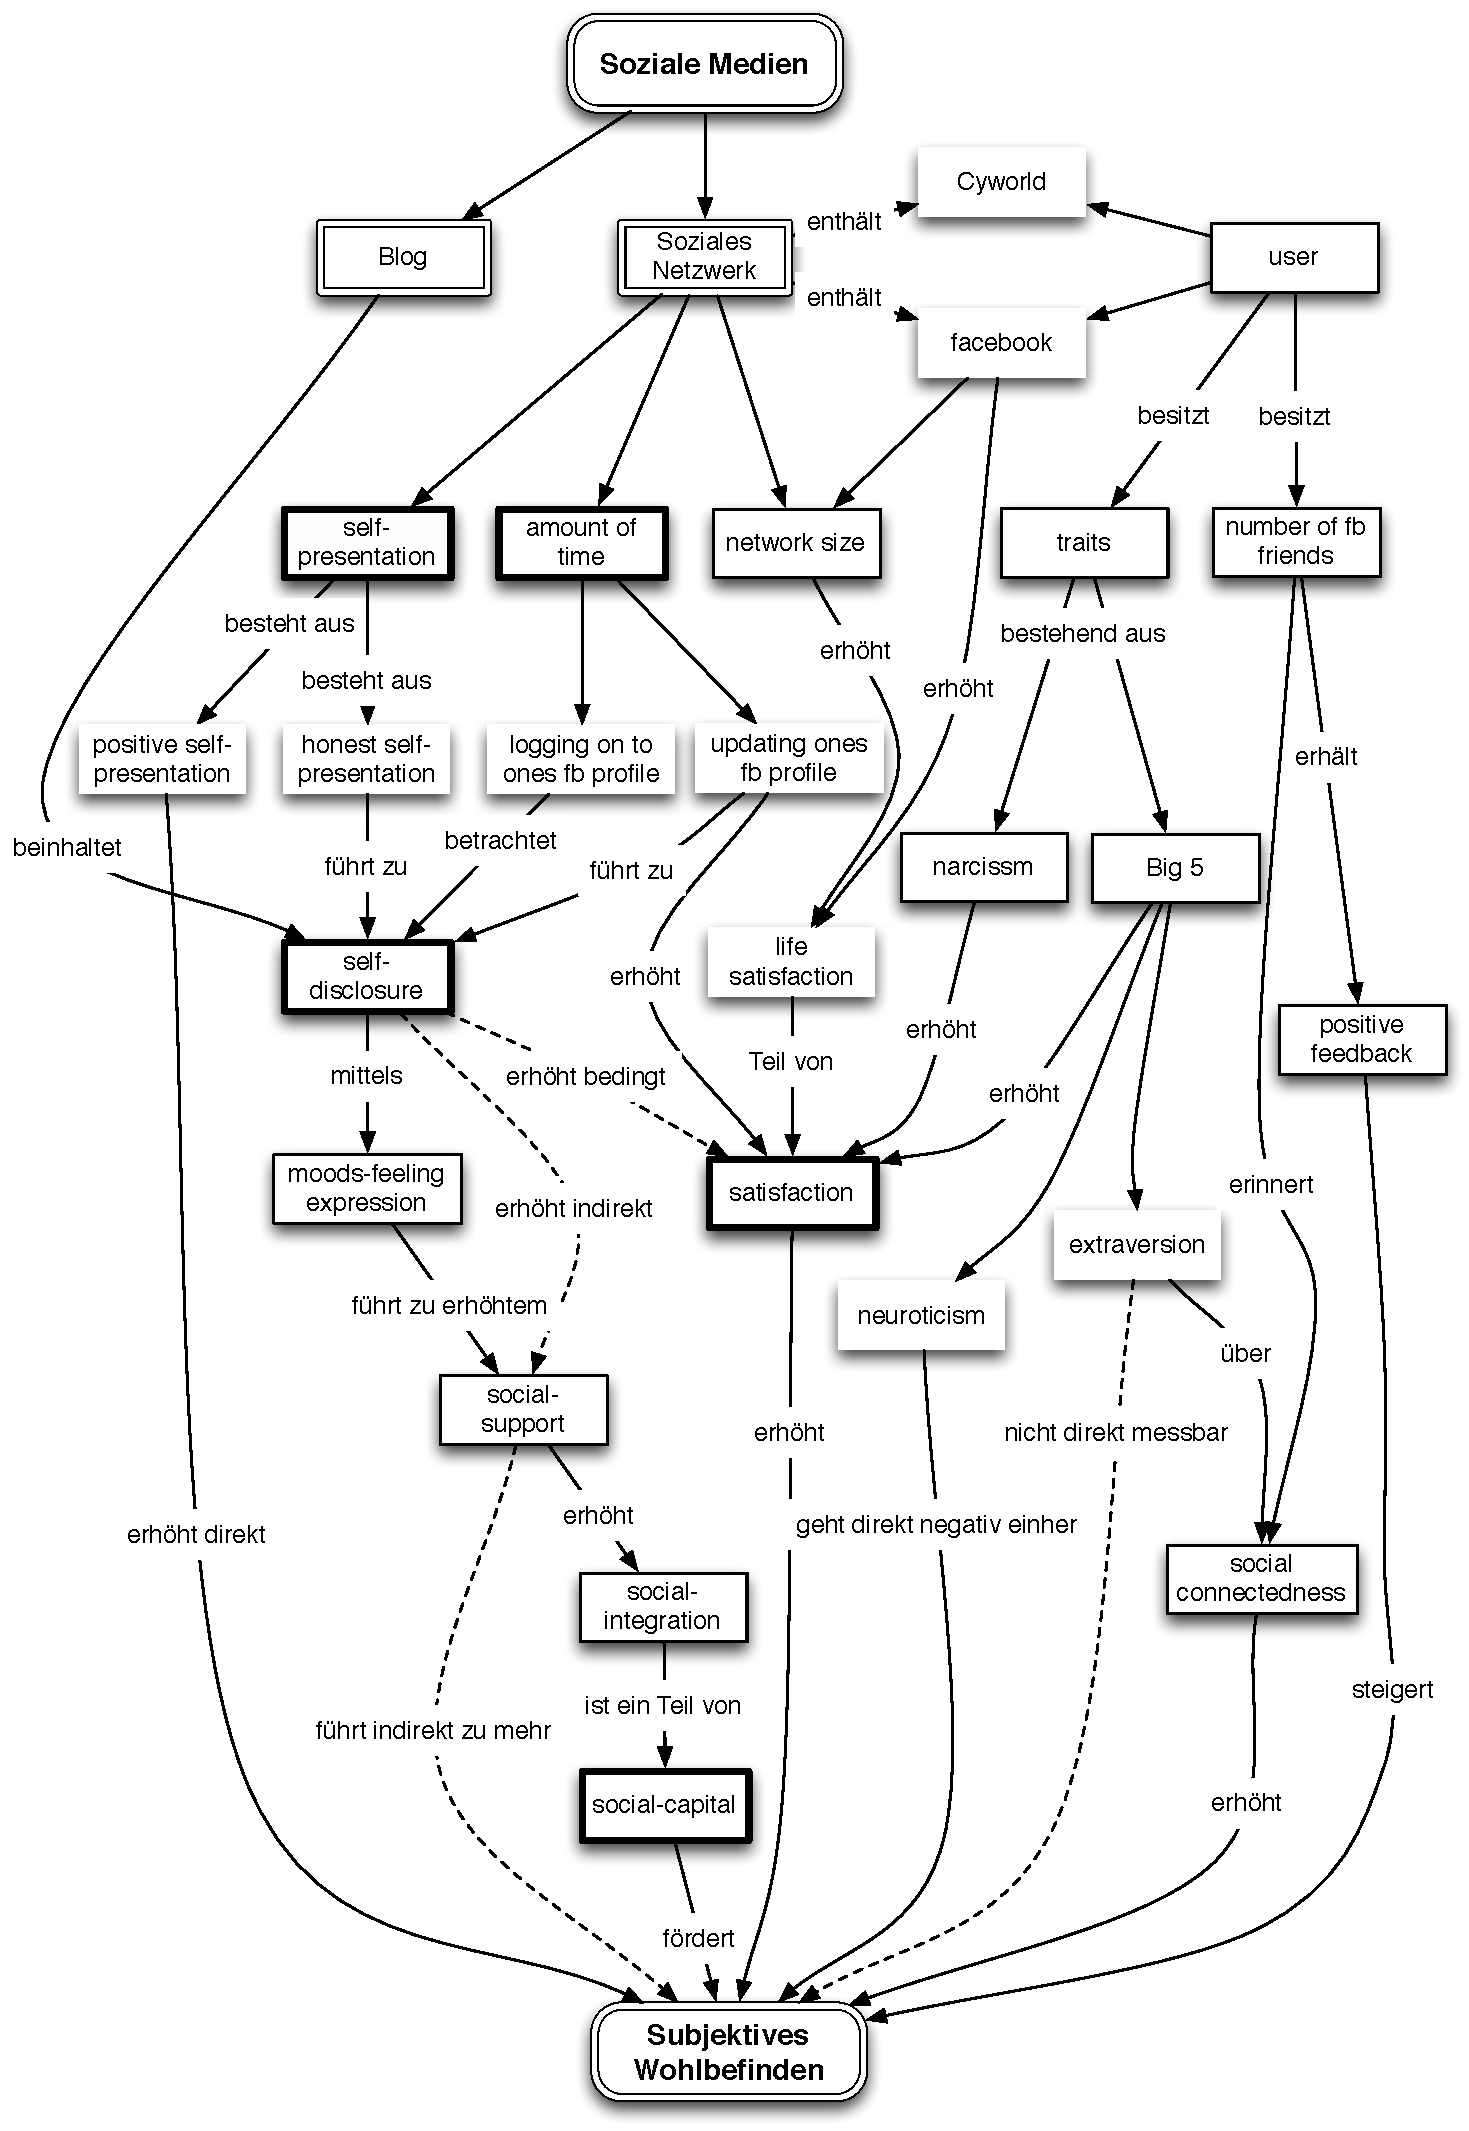
\includegraphics[width=0.4\textwidth]{images/grafiken/conceptMap_Swb_Sm_v2.pdf}
	\caption{ConceptMap - Subjektives Wohlbefinden und Soziale Medien}
	\label{fig.ConceptMapSwbSm}
\end{figure} \newline
Die Grafik stellt einen Zusammenzug unterschiedlicher Studien dar, die sich mit den Auswirkungen von \gls{sm} auf das \gls{swb} auseinander setzen. Darin sind die verschiedenen Konstrukte ersichtlich, die in den Studien verwendet wurden. Gelesen wird die Grafik ausgehend von den \gls{sm} entlang den Verbindungslinien bis hin zum \gls{swb}.\newline
Innerhalb der Grafik wurden die Englischen Begriffe aus den Studien übernommen. Bei den Verbindungslinien wurde mit Deutschen Wörtern gearbeitet.\newline
In den folgenden Unterkapiteln werden diese Konzepte anhand der Grafik erläutert. Dazu wird die Grafik in verschiedene Stränge unterteilt, um den komplexen Informationsgehalt in übersichtliche Häppchen aufzuteilen. Die Stränge sollen von den \gls{sm} ausgehend, über wichtige Konzepte und Begriffe, bis hin zum \gls{swb} führen. Da es sich um eine komplexe Thematik handelt, ist es nicht immer möglich die Grenzen scharf zu ziehen. Viele Konzepte überschneiden sich und greifen ineinander über.\newline 
Die in der Grafik markierten Konzepte und Begriffe werden in den folgenden Kapiteln näher erläutert. Wo dies möglich ist, werden die englischen Begriffe ins Deutsche übersetzt. Für Begriffe, bei denen die ursprüngliche Bedeutung durch einen unsachgemässe Übersetzung gefährdet ist, oder das deutsche Pendant dazu fehlt oder unklar ist, wird das originale englische Wort verwendet. Bei den jeweiligen Worterklärungen wird dem Englischen Begriff eine mögliche Deutsche Übersetzung mitgeliefert, wobei hier zu beachten ist, dass die Begriffe in den Studien nicht immer identisch verwendet werden und die Bedeutung je nach Verwendung des Autors leicht abweichen kann.

%UK Self-Presentation, Self-dicslosure und social capital
%----------------------------------------------------------------------
\section{Selbstdarstellung, Selbstoffenbarung und Soziales Kapital}\label{sub.selfp}
In diesem Kapitel wird auf den Einfluss von Selbstdarstellung, Selbstoffenbarung und Soziales Kapital als Haupteinflussgrössen auf das \gls{swb} eingegangen. \newline
Unter \textbf{Selbstdarstellung} (engl. self-presentation) wird eine Strategie verstanden, die im Kontext von Facebook näher untersucht wurde \cite{Kim:2011}. Facebook stellt nicht nur Mechanismen zur Verfügung, um Benutzerverbindungen untereinander grafisch darzustellen, sondern auch technologische Möglichkeiten, wie sich Benutzer selber darstellen können \cite{Ellison:2007.1}. Je nach dem welche Möglichkeiten ein Benutzer verwendet (z.B.: Statusaktualisierung, erstellen und pflegen eines Fotoalbums, Nachrichten auf dem eigenen Profil posten, etc.) stellen sich diese Benutzer unterschiedlich getreu dar. In der Literatur wird zwischen zwei unterschiedlichen Strategien innerhalb der Computervermittelten Kommunikation (engl. Computer-mediated communication) \cite{Tidwell:2002} und Selbstdarstellung auf online Partnervermittlungsplattformen \cite{Gibbs:2006}  unterschieden: Positive- und ehrliche Selbstdarstellung. Auf der einen Seite wird eine hohe Aktivität eines Benutzers auf Facebook ihn dazu bewegen, sich möglichst positiv darzustellen \cite{Kimmerle:2008} und auf der anderen Seite werden sich Benutzer, die eine langfristige Beziehung anstreben, sich eher auf eine ehrliche Art präsentieren \cite{Gibbs:2006}. Die Frage stellt sich, ob eine positive und ehrliche Darstellung der eigenen Person auf Facebook einen Einfluss auf das \gls{swb} hat.\newline
Im Gegensatz zur Darstellung eines Individuums, wie es auf Facebook erfolgt, werden auf einem Journal oder Blog eigentliche Texte veröffentlicht. Ein persönliches Journal widerspiegelt die innere Welt eines Autors, was unter dem Begriff \textbf{Selbstoffenbarung} (engl. self-disclosure) verstanden wird. Ein Prozess, bei dem ein Individuum sein Gefühle, Gedanken, Erlebnisse und Informationen mit anderen Personen teilt \cite{Derlega:1993}. Baker und Moore gehen davon aus \cite{Baker:2008}, dass die Selbstoffenbarung dazu beitragen kann, existierende Beziehungen aufrecht zu erhalten und das eigene Beziehungsnetzwerk auszubauen. Beide Vorgänge werden gemäss Putnam \cite{Putnam:2000} als wichtige Faktoren für das \textbf{Soziale Kapital} (engl. social capital) benötigt, welches erheblich zur Erhöhung des \gls{swb} beisteuert \cite{Sirgy:2006}. Unter Sozialem Kapital werden Beziehungen verstanden, die sich aus virtuellen und realen Beziehungen zusammensetzen \cite{Ellison:2007} und wird als Netzwerkphänomen angesehen. Die Zugehörigkeit zu einer Gruppe lässt sich als Ressource auffassen, die es einem Akteur ermöglicht, sowohl für sich selbst als auch für die Gruppenmitglieder positive Auswirkungen zu erzielen \cite{Bourdieu:1983}.\newline
%SubSec Ergebnisse
Gemäss den Untersuchungen von \citeA{Kim:2011} hat die positive Selbstdarstellung einen direkten positiven Effekt auf das \gls{swb}. Aus dieser Studie geht hervor, dass Facebook-Benutzer glücklicher sind, wenn sie ihr Selbstbild durch eine positive Selbstdarstellung bekräftigen und unterstützen. Dieses Ergebnis wird durch die 'positive illusion theorie' von Taylor zusätzlich gestützt \cite{Taylor:1996,Taylor:1988}. Diese Theorie besagt, dass eine voreingenommene Erkenntnis über das Ich oder eine Erkenntnis, die durch eine Erhöhung des eigenen Ansehens entstanden ist, helfen kann mit stressvollen oder bedrohlichen Situationen besser umzugehen und sich dadurch glücklicher zu fühlen (engl. feel happy). \newline
Im Gegenzug wirkte sich die ehrliche Selbstdarstellung bei \citeA{Kim:2011} indirekt positiv auf das \gls{swb} aus, in dem die soziale Unterstützung aus dem Umfeld erhöht wahrgenommen wird. Dieses Ergebnis unterstreicht die Wichtigkeit des Konzepts der Selbstoffenbarung, welches das Schlüsselement bei der Entwicklung von sozialen Online-Beziehungen darstellt \cite{Joinsen:2001}. Facebook-Freunde sind eher gewillt ihresgleichen zu helfen, wenn diese Person das Bedürfnis über angemessene Selbstoffenbarung kommuniziert und sich durch eine ehrliche Selbstdarstellung auf Facebook präsentiert. Diese Unterstützung durch das soziale Umfeld führt zu einem förderlichen \gls{swb} \cite{Greene:2006}.\newline
Eine weitere Studie von \citeA{Ko:2009} belegt, dass sich das Benehmen von Blogger durch Selbstoffenbarung signifikant und direkt auf die soziale Integration und dadurch auf das Soziale Kapital auswirkt, welches wiederum das \gls{swb} der Blogger erhöht. Erklärt wird dieses Phänomen dadurch, dass in den meisten publizierten Artikeln die Launen und Gefühle der Blogger eine entscheidende Rolle spielen. 93\% der Blogger geben an, dass der Ausdruck von Stress, Hemmungen, Druck und Verstimmungen in ihren Artikeln ausgedrückt werden \citeyear<ebda.,>{Ko:2009}. Diese Angaben decken sich mit den Resultaten von \citeA{Pennebaker:1997}, die besagen, dass wenn Menschen ihre Gedanken zu ihren Launen und Gefühlen mit anderen Menschen durch Schreiben mitteilen, dies zu einer grösseren Unterstützung durch das soziale Umfeld und demzufolge zu einer höheren sozialen Integration führt. Der soziale Support wird des Weiteren mit einer aktiven Nutzung von persönlichen Blogs in Verbindung gesetzt \cite{Jung:2012}. Aktive Blogg-Nutzer, die selber Texte schreiben und lesen, werden den Einfluss von sozialen Support eher zu spüren bekommen, als solche, die Blogs nur selten nutzen. Die soziale Integration wiederum ist ein Teil des Sozialen Kapitals, welches eine Erhöhung des \gls{swb} voraussagt \cite{Ko:2009}. \newline
Die soeben genannten Faktoren werden von der Studie von \citeA{Lee:2011} weiter gestützt. Die Menge an Selbstoffenbarung eines Benutzers in Sozialen Netzen geht positiv mit dem \gls{swb} einher. Benutzer, die sich selber sehr stark einer Selbstoffenbarung unterziehen, erwarten ebenso eine Selbstoffenbarung von Seiten ihrer Freunde. Ebenso erwarten diese Benutzer ein gewisses Mass an sozialer Unterstützung.\newline
Zusammenfassend aus den oben erwähnten Studien geht hervor, dass der Einfluss von \gls{sm} mittels Selbstdarstellung, Selbstoffenbarung und dem Sozialen Kapital einen positiven Einfluss auf das \gls{swb} haben.

%UK Summe der verwendeten Zeit (amount of time)
%----------------------------------------------------------------------
\section{Aufgewendete Zeit und Befriedigung} \label{sub.amount}
Dieses Kapitel beschäftigt sich mit dem Einflussfaktor der aufgewendeten Zeit, die ein Benutzer mit \gls{sm} verbringt und der Befriedigung, welche durch die Benutzung von \gls{sm} erlangt wird. \newline
Die \textbf{aufgewendete Zeit} (engl. amount of time), die ein durchschnittlicher \gls{sm}-Benutzer täglich im Netz verbringt variiert von Studie zu Studie. Je nach dem, wann diese Studie durchgeführt wurde, unterscheidet sich die Nutzungsdauer erheblich. So wurde die durchschnittliche tägliche Nutzung von Facebook bei \citeA{Cassidy:2006} mit 10 bis 30 Minuten angegeben. Aus einer aktuellen Statistik ist zu entnehmen, dass die durchschnittliche Nutzung von \gls{sm} im Allgemeinen in etwa 16 Minuten beträgt \cite{Bannon:2012}. Wobei die durchschnittliche Nutzung von Facebook im Jahre 2012 mit etwas über 20 Minuten im Tag weltweit angegeben wird \cite{Pring:2012}.\newline
Unter \textbf{Befriedigung} (engl. satisfaction) wird ein Hauptmotiv verstanden, das für das schnelle Wachstum und die immense Popularität von \gls{sm} verantwortlich scheint \cite{Special:2012}. Dabei setzt sich die Befriedigung aus den Bemühungen für die Personalisierung des eigenen Benutzerkontos und eines möglichen gesellschaftlichen Gewinns, durch die Nutzung von \gls{sm} zusammen \cite{Aronson:1959}. Es wird zudem angenommen, dass ein weiterer Motivationsfaktor im Zusammenhang mit dem Grad der Selbstoffenbarung zu finden ist, wobei die Selbstoffenbarung mit der Befriedigung von Bedürfnissen, eigene Ziele zu erreichen, einhergeht \cite{Special:2012}. Diverse Studien haben einen positiven Zusammenhang zwischen der Nutzung von Facebook und der Lebenszufriedenheit (engl. life satisfaction) hergestellt \cite<z.B.,>{Ellison:2007,Valenzuela:2009}. \newline
%SubSec Ergebnisse
Gemäss \citeA{Special:2012} führen zwei Gründe zu einer erhöhten Befriedigung durch die Nutzung von Facebook: Einerseits führt die reine aufgewendete Zeit, für das Erstellen und das Warten des eigenen Facebook-Kontos, direkt zu einer Befriedigung. Andererseits führt der Wunsch, sich anderen Facebook-Benutzer in einem möglichst begehrenswerten Selbstbild zu präsentieren, zu einer gesteigerten Befriedigung. Die Resultate dieser Studie zeigen, je mehr Zeit für die Pflege und Wartung der eigenen Seite verwendet wird, desto grösser ist die empfundene Befriedigung. Hingegen verspüren Benutzer eine geringere Befriedigung, die sich nur ab und zu auf Facebook anmelden, um damit ihre Freizeit verbringen. \newline
Benutzer, die einen hohen Grad an Selbstoffenbarung zeigen, spüren vor allem eine Befriedigung bei der Nutzung von Facebook als Unterhaltungsmethode und Freizeitbeschäftigung. Offen in dieser Studie bleibt die Frage, ob es einen direkten Zusammenhang zwischen dem Grad der Selbstoffenbarung und einer erhöhten Befriedigung gibt.\newline
Gemäss \citeA{Lee:2011} konnte kein Zusammenhang zwischen der wöchentlichen Nutzungszeit von Sozialen Netzwerken und einer erhöhten Befriedigung hergestellt werden. Dafür konnten sie einen direkten Einfluss zwischen der Grösse eines Sozialen Netzwerks und der Lebenszufriedenheit aufzeigen. Diese These wird durch die Studie von \citeA{Manago:2012} gestützt, in der die Teilnehmer über eine Zunahme von Lebenszufriedenheit und sozialer Unterstützung berichteten, je grösser die verwendete Platform und die Menge, der darin zu erreichenden Personen ist (in Abbildung ~\ref{fig.ConceptMapSwbSm} wurde die Verbindung zwecks Übersicht zwischen Lebenszufriedenheit und sozialem Support weggelassen). 

%UK Benutzer Traits
%----------------------------------------------------------------------
\section{Benutzer Eigenschaften und Anzahl Facebook-Freunde}\label{sub.traits}
Dieses Kapitel befasst sich mit den Auswirkungen von persönlichen Eigenschaften (traits), die eine Person mit sich bringt und der Anzahl von Facebook-Freunden, mit denen ein Benutzer mittels \gls{sm} verbunden ist.\newline
%SubSec Einführung
Der Einfluss von \textbf{Persönlichkeitsfaktoren} (engl. traits) auf das \gls{swb} ist anhand von verschiedenen Meta-Analysen nachgewiesen worden \cite<z.B.,>{Diener:1999,Steel:2008}. Wobei vor allem die beiden Grössen Extraversion und Neurotizismus aus dem Fünf-Faktoren-Modell (engl. Big-Five) einen erhöhten Einfluss auf das eigene Glücksempfinden ausüben. Aus neuropsychologischer und verhaltenstheoretischer Sicht stehen diese persönlichen Eigenschaften in direktem Verhältnis zum \gls{swb} \cite{Emmons:1985}. Als Beispiel zur Verdeutlichung: Extravertierte Personen verwenden viel Zeit und Aufwand im Pflegen von Beziehungen und schätzen die Belohnung, die durch den zwischenmenschlichen Austausch hervorgeht \cite{Lee:2011}. Neurotisch veranlagte Personen neigen dazu sich Sorgen im alltäglichen Leben zu machen, was zu erhöhter depressiven Verstimmungen und erhöhter Ängstlichkeit führt (ebda.,2011). Je nach Ausprägung dieser beiden Persönlichkeitsdimensionen, wird eine unterschiedliche Motivation in der Verwendung von Sozialen Netzwerken zugeschrieben \cite<z.B.,>{Amiel:2004,Hamburger:2000}. \citeA{Sheldon:2008} führt auf, dass introvertierte Benutzer sich eher wohl fühlen könnten durch die Kommunikation über das Internet, als im physischen Leben. Obwohl auch Sheldon in seiner Studie darauf verweist, dass diejenigen Menschen, die eine rege Online-Kommunikation betreiben, auch im wirklichen Leben zu einer aktiveren Kommunikation neigen.\newline
Gemäss \citeA{Twenge:2008} wurde in den vergangenen Jahren, zeitgleich zur stetigen Entwicklung der Sozialen Netzen, ein Anstieg von Personen mit einer narzisstischen Persönlichkeitseigenschaft festgestellt. Narzissmus als Persönlichkeitskonstrukt ist gekennzeichnet durch ein Gefühl der Einzigartigkeit, Selbstverherrlichung, der Unfähigkeit Kritik entgegenzunehmen und der Erwartung, Leistungen ohne entsprechende Gegenleistung zu bekommen \cite{Raskin:1988}. Diese Eigenschaften werden durch exhibitionistischen Tendenzen, Eitelkeit, Versenkung in sich selber und Überlegenheitsgefühlen ergänzt \cite{Ackerman:2011}. Ob und wie sich diese Eigenschaft auf das \gls{swb} auswirkt, ist Ziel der Studie von \citeA{Carpenter:2012}.\newline
Die durchschnittliche Anzahl der Facebook-Freunden nahm in den vergangen Jahren kontinuierlich zu. Von durchschnittlich 137 Freunden im Jahre 2006 \cite{Subrahmanyam:2008}, über 185 im Jahr 2007 \cite{Manago:2008} bis 440 Facebook-Freunde im Jahr 2009 \cite{Manago:2012}. Verschieden Studien haben versucht, den Zusammenhang zwischen \gls{swb} und Anzahl Facebook-Freunde herzustellen \cite<z.B.,>{Ellison:2007,Valenzuela:2009}. \newline
%SubSec Ergebnisse
Gemäss den Studien von \citeA{Lee:2011} geht die Persönlichkeitseigenschaft Neurotizismus negativ einher mit \gls{swb}. Wo hingegen bei Extraversion kein signifikanter Zusammenhang im Bezug auf das \gls{swb} ausgemacht werden konnte. Vermerkt sei hier, dass die Beziehung zwischen Extraversion und \gls{swb} sehr komplex ist. Denn obwohl extravertierte Personen öfters gesellschaftliche Kontakte knüpfen und durch zwischenmenschliche Beziehungen einen Nutzen ziehen, gehen sie öfters ein höheres Risiko ein, was sich negativ auf die Weiterentwicklung im evolutionären Kontext auswirkt \cite{Nettle:2005}. Auf ein ähnliches Ergebnis kommt die Studie von \citeA{Lee:2008}, die den Zusammenhang zwischen Extraversion und \gls{swb} zu ermitteln versucht. Der Zusammenhang ist nicht direkt ersichtlich, sondern stellt sich über die soziale Verbundenheit (engl. social connectedness) ein.\newline
\citeA{Special:2012} vermuten einen Zusammenhang zwischen Narzissmus und Befriedigung. Sie gehen davon aus, dass Personen mit einem narzisstischen Zug, eine weitere Möglichkeiten für die gewünschte Selbstbewunderung auf Sozialen Netzen zur Verfügung steht, was zu einer Zunahme der Befriedigung führt. Die Studie von \citeA{Manago:2012} hingegen wirft die Frage auf, ob die Netzwerkgrösse mit dem Selbstwert der Benutzer zusammenhängt. Wird nämlich, so die Autoren, der Selbstwert durch die Grösse der Sozialen Netze gesteigert, könnte dies mit einer Überhöhung des Selbstwertes und einer Vergrösserung des narzisstischen Persönlichkeit einhergehen, was auch von der Studie um \citeA{Twenge:2008} gestützt wird. Personen die sich gerne als grossartig Darstellen, treiben einen enormen Aufwand, sich einer grossen Öffentlichkeit zu präsentieren \cite{Carpenter:2012}. Diese Personen suchen nach gesteigerter sozialen Unterstützung, ohne diese selber anzubieten. \newline
Ebenso konnte \citeA{Lee:2011} einen positiven Zusammenhang zwischen der Anzahl Facebook-Freunde und \gls{swb} herstellen. Die Autoren gehen jedoch davon aus, dass es keinen direkten Zusammenhang dazwischen gibt, sondern dass der Benutzer, durch die ersichtlichen Freunde, an die soziale Verbundenheit erinnert wird und das \gls{swb} dadurch indirekt eine Steigerung erfährt. Sie konnten zudem eine negative Assoziation zwischen der Anzahl Facebook-Freunde und der wahrgenommener sozialer Unterstützung erstellen (in der Abbildung ~\ref{fig.ConceptMapSwbSm} nicht eingezeichnet). Begründet wird diese Feststellung dadurch, dass  die Pflege von nahe Beziehungen Zeit und Aufwand benötigt und Personen mit vielen Online-Freunden eben diese Zeit nicht besässen und sie deshalb vernachlässigen.\newline
Eine holländische Studie über junge Erwachsene fand heraus, dass positive Rückmeldungen (engl. positive feedback) der Sozialen Netzwerk-Freunde, das wahrgenommene \gls{swb} steigern. Wobei die soziale Unterstützung durch diese Freunde mit der Nutzungshäufigkeit von Sozialen Netzen und dem \gls{swb} einhergehen \cite{Valkenburg:2006}. 



% Diskussion
%%%%%%%%%%%%%%%%%%%%%%%%%%%%%%%%%%%%%%%%%%%%%%%%%%%%%%%%%%%%%%%%%
%  _____   ____  _____                                          %
% |_   _| /  __||  __ \    Institute of Computitional Physics   %
%   | |  |  /   | |__) |   Zuercher Hochschule Winterthur       %
%   | |  | (    |  ___/    (University of Applied Sciences)     %
%  _| |_ |  \__ | |        8401 Winterthur, Switzerland         %
% |_____| \____||_|                                             %
%%%%%%%%%%%%%%%%%%%%%%%%%%%%%%%%%%%%%%%%%%%%%%%%%%%%%%%%%%%%%%%%%
%
% Project     : LaTeX doc Vorlage für Windows ProTeXt mit TexMakerX
% Title       : 
% File        : diskussion.tex Rev. 00
% Date        : 7.5.12
% Author      : Remo Ritzmann
% Feedback bitte an Email: remo.ritzmann@pfunzle.ch
%
%%%%%%%%%%%%%%%%%%%%%%%%%%%%%%%%%%%%%%%%%%%%%%%%%%%%%%%%%%%%%%%%%

\chapter{Diskussion und Ausblick}\label{chap.diskussion}

\begin{itemize}
\item Eingehen auf die Gefahren von SM (auch wenn Umfang nicht reichte, dies in der Arbeit einfliessen zu lassen), ev Buch von Digitaler Demenz erwähnen
\item 
\end{itemize}


% Literaturverzeichnis
%%%%%%%%%%%%%%%%%%%%%%%%%%%%%%%%%%%%%%%%%%%%%%%%%%%%%%%%%%%%%%%%%
%  _____   ____  _____                                          %
% |_   _| /  __||  __ \    Institute of Computitional Physics   %
%   | |  |  /   | |__) |   Zuercher Hochschule Winterthur       %
%   | |  | (    |  ___/    (University of Applied Sciences)     %
%  _| |_ |  \__ | |        8401 Winterthur, Switzerland         %
% |_____| \____||_|                                             %
%%%%%%%%%%%%%%%%%%%%%%%%%%%%%%%%%%%%%%%%%%%%%%%%%%%%%%%%%%%%%%%%%
%
% Project     : LaTeX doc Vorlage für Windows ProTeXt mit TexMakerX
% Title       : 
% File        : literatur.tex Rev. 00
% Date        : 23.4.12
% Author      : Remo Ritzmann
% Feedback bitte an Email: remo.ritzmann@pfunzle.ch
%
%%%%%%%%%%%%%%%%%%%%%%%%%%%%%%%%%%%%%%%%%%%%%%%%%%%%%%%%%%%%%%%%%

\begin{thebibliography}{99}
\addcontentsline{toc}{section}{Literaturverzeichnis}\label{cha:literaturverzeichnis}

% How to make a Literaturlist nach www.ieee.org/documents/ieeecitationref.pdf
% Erklärung

%Books
\bibitem{robotvision} B. Klaus and P. Horn, Robot Vision. Cambridge, MA: MIT Press, 1986.
%Einzelne Seiten aus Buch
\bibitem{randompatterns} L. Stein, ">Random patterns,"> in Computers and You, J. S. Brake, Ed. New York: Wiley, 1994, pp. 55-70.

%Reports

% Peridicals (Zeitschriften)



% Gibt es eine automatische Konvertierung von Bibtech to LaTeX?

% Alte Beispiele
\bibitem{miktex} Latex Programmiere Umgebung (basic-miktex-2.8.3582.exe)\\
\href{http://www.miktex.org/about}{miktex.org}, 28.03.2010

\bibitem{wireshark}Wireshark, Programm zur Darstellung von Ehternet Packeten\\
\href{http://www.wireshark.org/download.html}{http://www.wireshark.org/download.html}



\end{thebibliography}


% Anhang
%%%%%%%%%%%%%%%%%%%%%%%%%%%%%%%%%%%%%%%%%%%%%%%%%%%%%%%%%%%%%%%%%
%_____________ ___    _____  __      __ 
%\____    /   |   \  /  _  \/  \    /  \  Institute of Applied
%  /     /    ~    \/  /_\  \   \/\/   /  Psychology
% /     /\    Y    /    |    \        /   Zuercher Hochschule 
%/_______ \___|_  /\____|__  /\__/\  /    fuer Angewandte Wissen.
%        \/     \/         \/      \/                           
%%%%%%%%%%%%%%%%%%%%%%%%%%%%%%%%%%%%%%%%%%%%%%%%%%%%%%%%%%%%%%%%%
%
% Project     : Seminararbeit
% Title       : 
% File        : anhang Rev. 00
% Date        : 10.10.2012
% Author      : Till J. Ernst
%
%%%%%%%%%%%%%%%%%%%%%%%%%%%%%%%%%%%%%%%%%%%%%%%%%%%%%%%%%%%%%%%%%

\pagenumbering{Roman}

\appendix
\chapter{Anhang}\label{chap.anhang}
\section{Glossar}\label{sec.glossar}
\begin{table}[ht] \centering
	%\caption{Klassifizierung}
	\begin{tabular}{b{4cm} m{11cm} }	
		\rowcolor{gray} 
		
		\textbf{Ausdruck} & \textbf{Definition} \\ 
		\textbf{Blog} & Kommt ursprünglich aus dem Wort 'Weblog', was soviel wie Webeintrag bedeutet und wurde eines Tages von einem Blogger (jemand der Einträge in Blogs vornimmt) ironischerweise in den Ausspruch 'we blog' (deutsch 'wir bloggen') umgewandelt. Seid diesem Zeitpunkt wird für diese Art von Web-Tagebuch das Wort Blog verwendet \cite{Kaplan:2012}.  \\ 
		\textbf{Tweet / Twitter} & Twitter gehört in die Kategorie 'Mikroblogging' und ermöglicht den Versand von telegrammartigen Kurznachrichten. Es handelt sich um ein Echtzeit-Informationsnetzwerk, welches die maximal 140 Zeichen langen Nachrichten ähnlich der Form eines Schneeballsystems versendet \cite{Twitter:2012}. \\ 
	
	\end{tabular}
	\label{tab:glossar}
\end{table}

\section{Grafik: Einfluss Subjektives Wohlbefinden}\label{sec.anhangGrafik}
\begin{figure}[H]
	\centering
		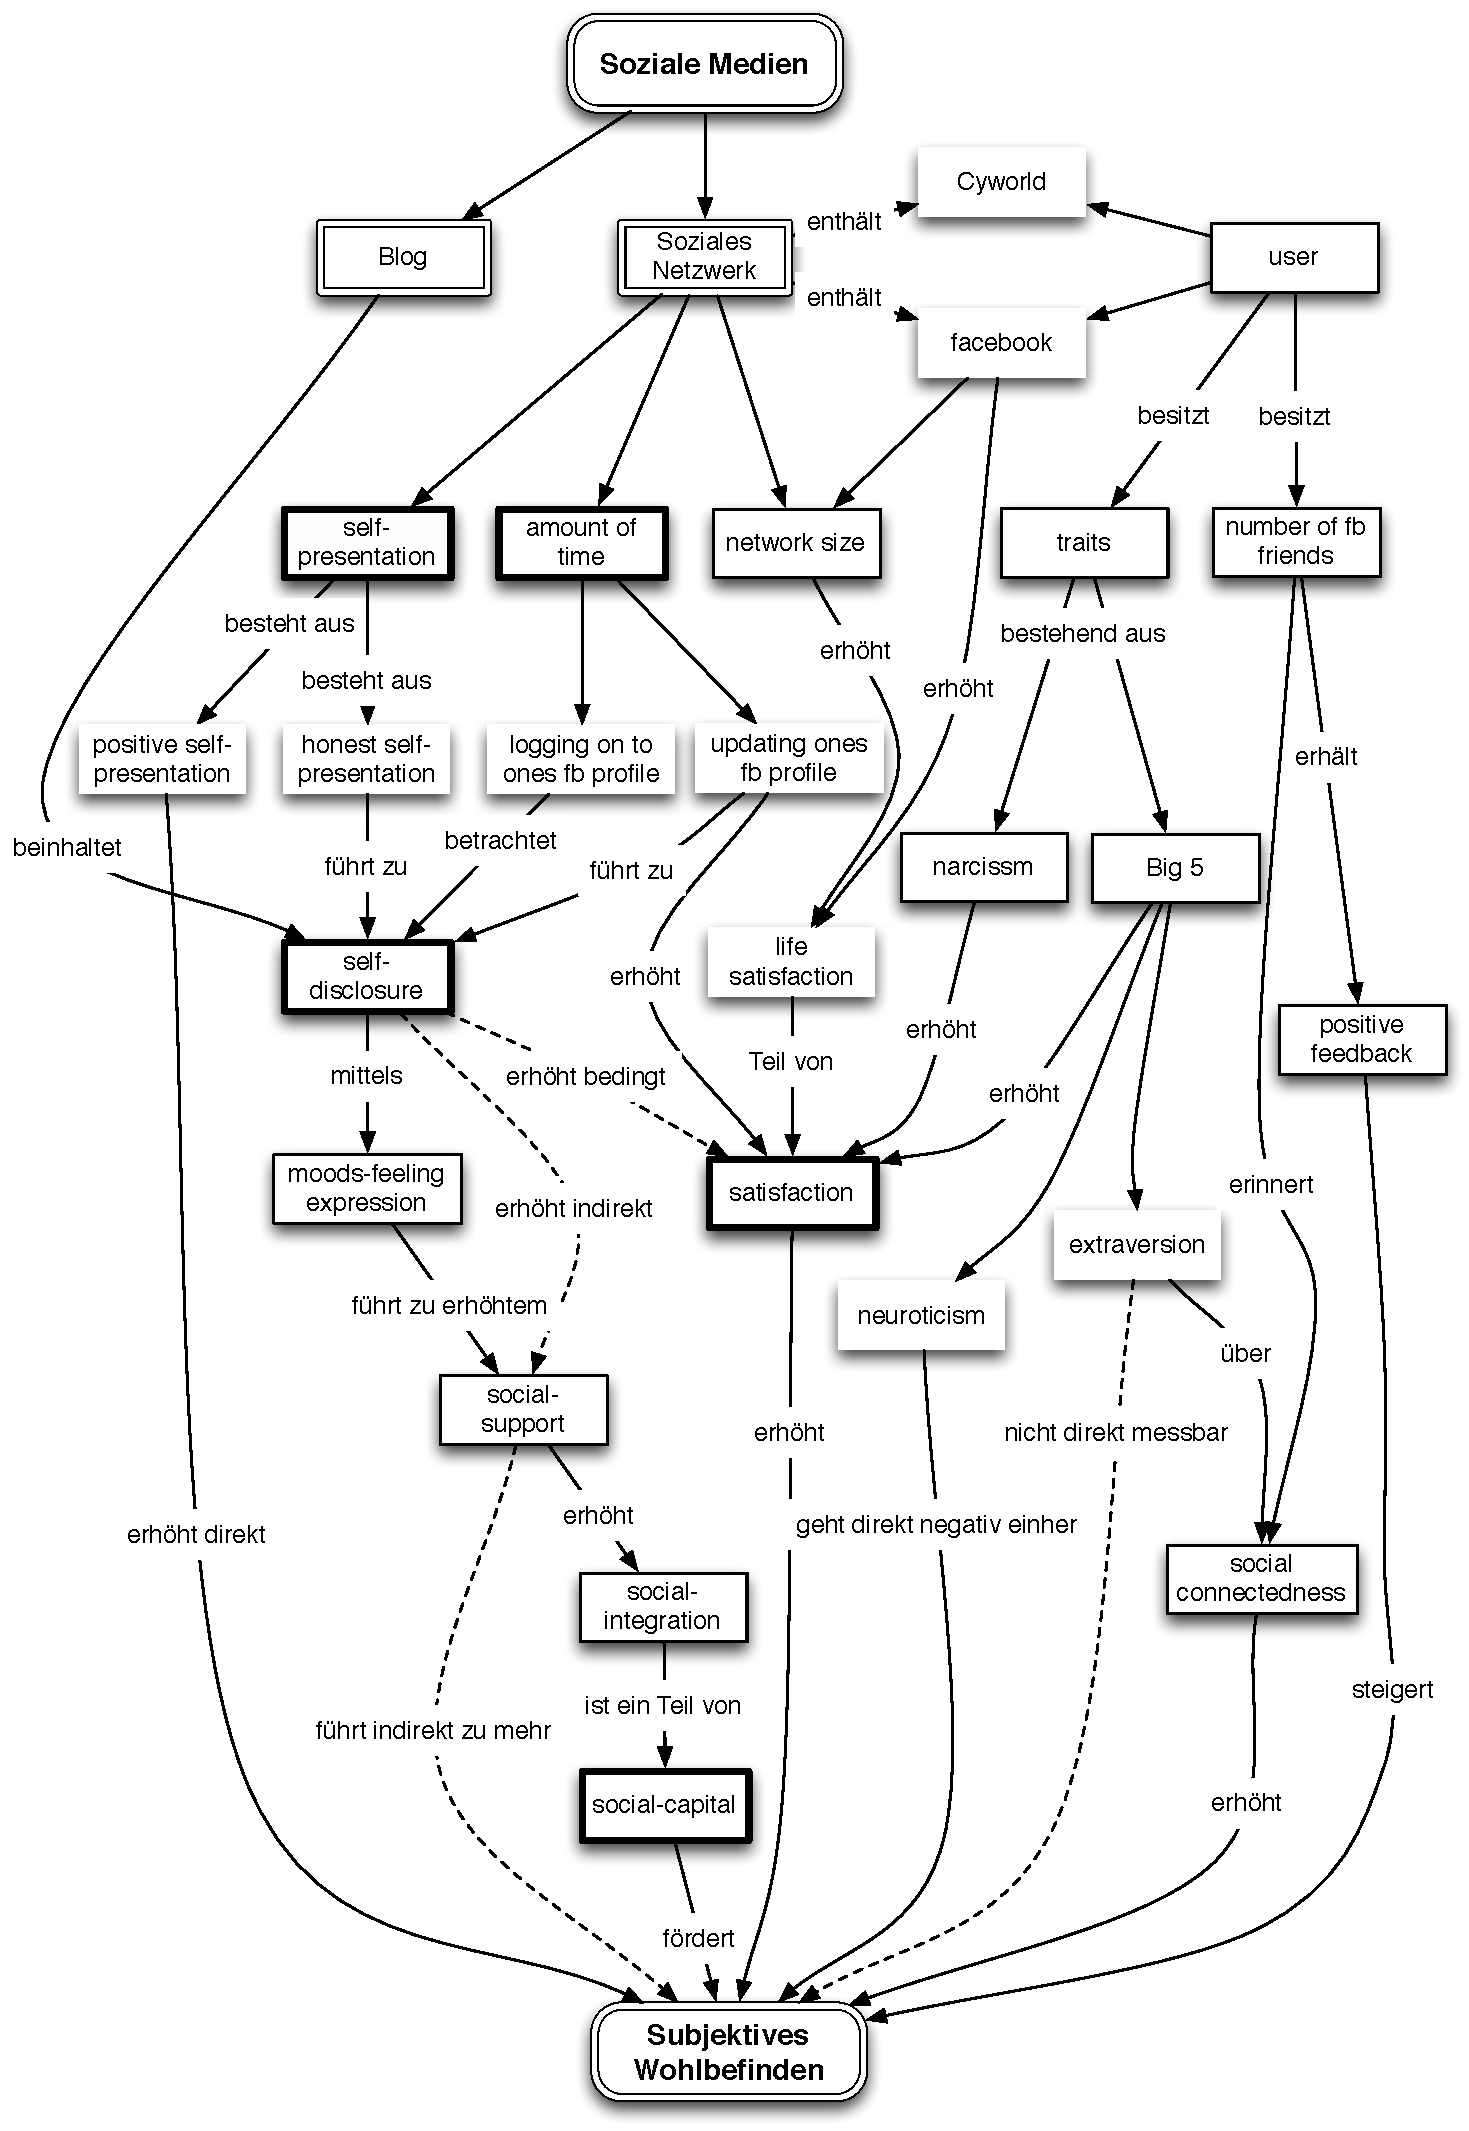
\includegraphics[width=0.9\textwidth]{images/grafiken/conceptMap_Swb_Sm_v2.pdf}
	\caption{ConceptMap - Subjektives Wohlbefinden und Soziale Medien}
	\label{fig.ConceptMapSwbSmAnhang}
\end{figure}


% Blatt mit Unterschrift

\includepdf{images/Seminararbeit_Unterschrift.pdf}

%%%%%%%%%%%%%%%%%%%%%%%%%%%%%%%%%%%%%%%%%%%%%%%%%%%%%%%%%%%%%%%%%
%  _____   ____  _____                                          %
% |_   _| /  __||  __ \    Institute of Computitional Physics   %
%   | |  |  /   | |__) |   Zuercher Hochschule Winterthur       %
%   | |  | (    |  ___/    (University of Applied Sciences)     %
%  _| |_ |  \__ | |        8401 Winterthur, Switzerland         %
% |_____| \____||_|                                             %
%%%%%%%%%%%%%%%%%%%%%%%%%%%%%%%%%%%%%%%%%%%%%%%%%%%%%%%%%%%%%%%%%
%
% Project     : LaTeX doc Vorlage für Windows ProTeXt mit TexMakerX
% Title       : 
% File        : header.tex Rev. 00
% Date        : 23.4.12
% Author      : Remo Ritzmann
% Feedback bitte an Email: remo.ritzmann@pfunzle.ch
%
%%%%%%%%%%%%%%%%%%%%%%%%%%%%%%%%%%%%%%%%%%%%%%%%%%%%%%%%%%%%%%%%%

\chapter{LaTeX Kurzanleitung}\label{chap.anleitung}
Dieses Kapitel führt mit Beispielcode in den LaTeX Code ein.\footnote{Verbesserungsvorschläge bitte an remo.ritzmann@pfunzle.ch senden}

Die nachfolgende Berichtstruktur wurde aus der Vorlage\footnote{Berichtstruktur Vorlage, Stand: August 2011} der \href{https://intra.zhaw.ch/departemente/school-of-engineering/studium-standort-winterthur/studierende/projektarbeit-bachelorarbeit.html}{PA/BA Termin-Webseite} vom ZHAW Intranet entnommen.

(): alle in Klammer aufgeführten Einträge sind situativ anzupassen



\section{Visio Vektorgraphik einfügen}\label{visio}
(Graphik auswählen) Speichern unter -> PDF -> Optionen.. -> Auswahl\\
Mit Adobe Akrobat öffnen: Erweitert -> Druckproduktion -> Seiten beschneiden -> Weisse Ränder entfernen -> OK -> Ctrl-S

\begin{figure}[H]
	\centering
		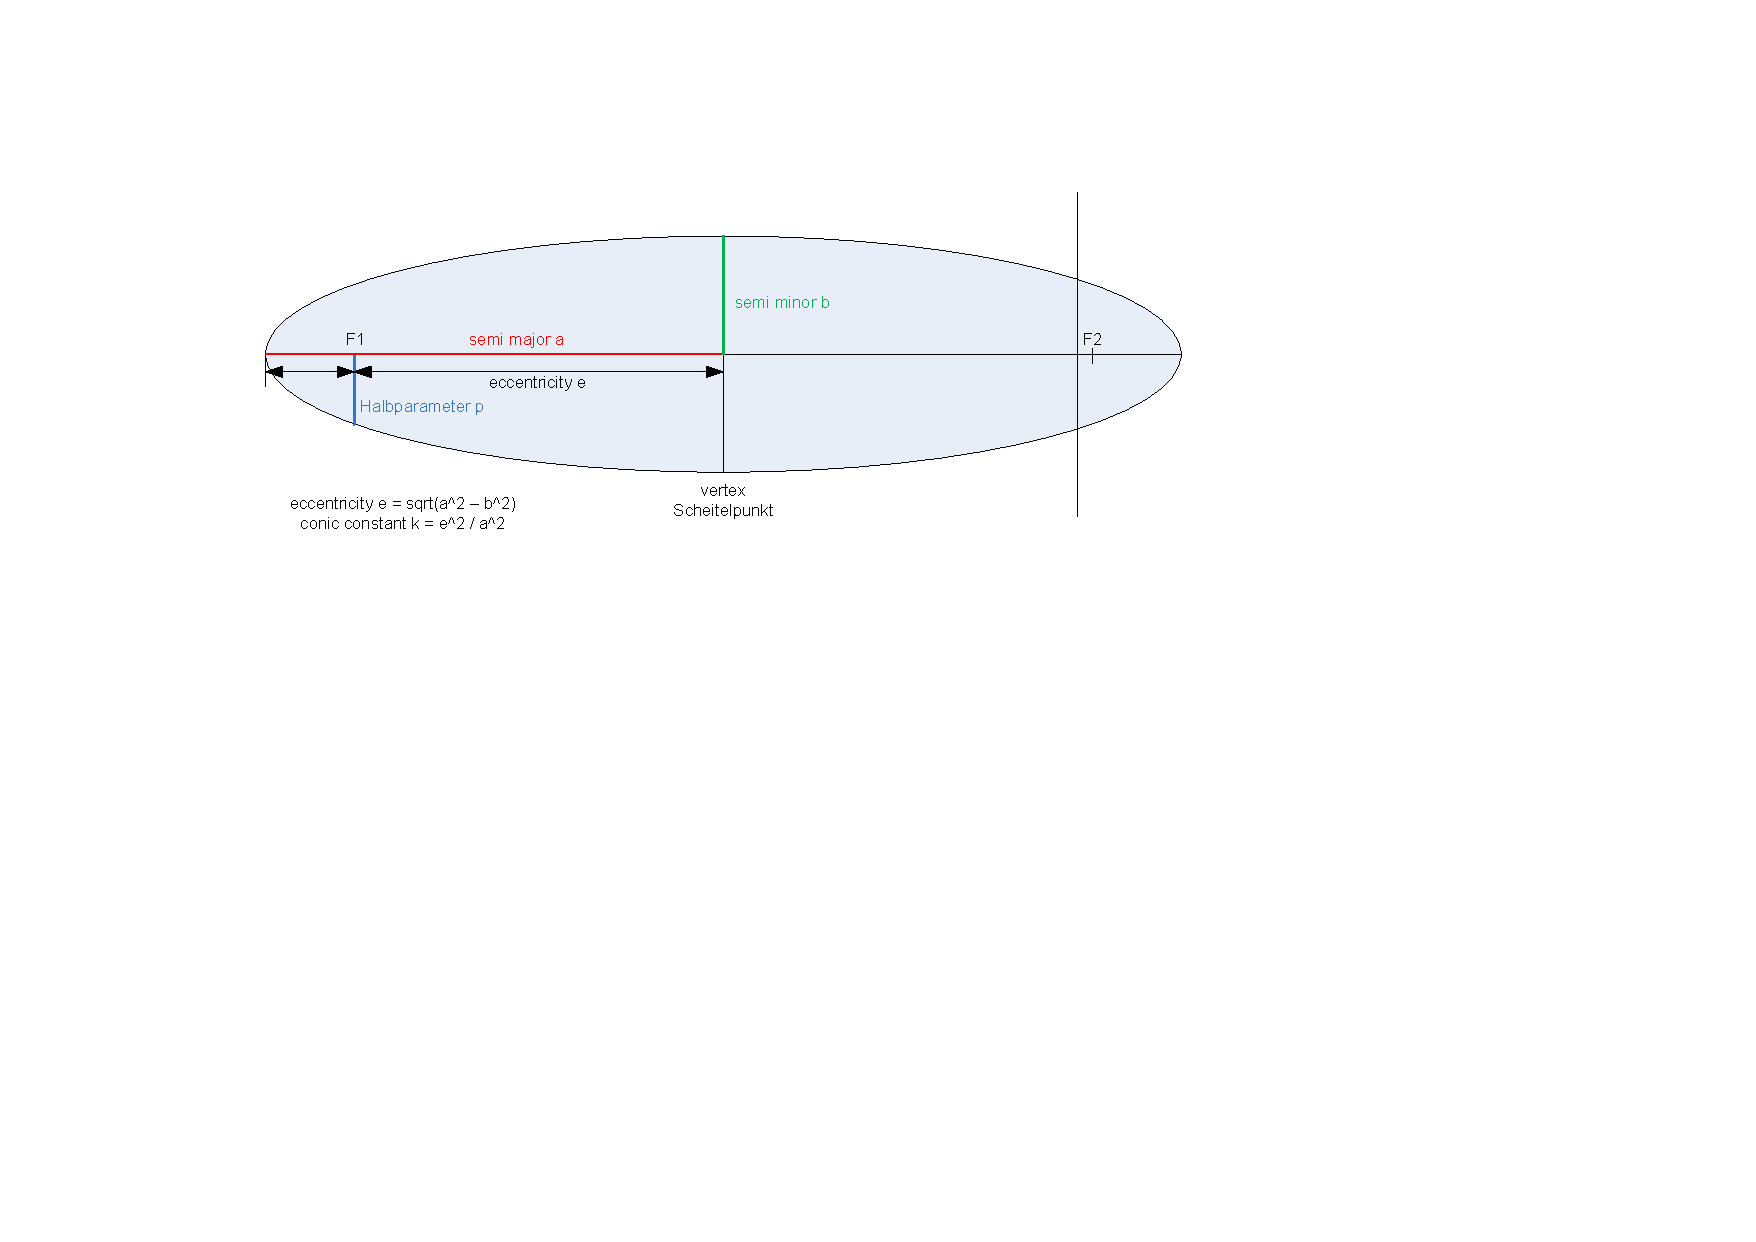
\includegraphics[width=0.8\textwidth]{images/visio/visio.pdf}
	\caption{Ideenskizze}
	\label{fig.Skizze}
\end{figure}

So kann die Abbildung~\ref{fig.Skizze} referenziert werden. Bei der PDF Erstellung ist darauf zu achten, dass LaTeX nur Versionen bis 1.4 voll unterstützt. 



\subsection{Graphiken in LaTeX zuschneiden}\label{zuschneiden}
Mit dem Befehl Clip kann eine Graphik auch in LaTeX zugeschnittenwerden:

\begin{figure}[H]
	\centering
		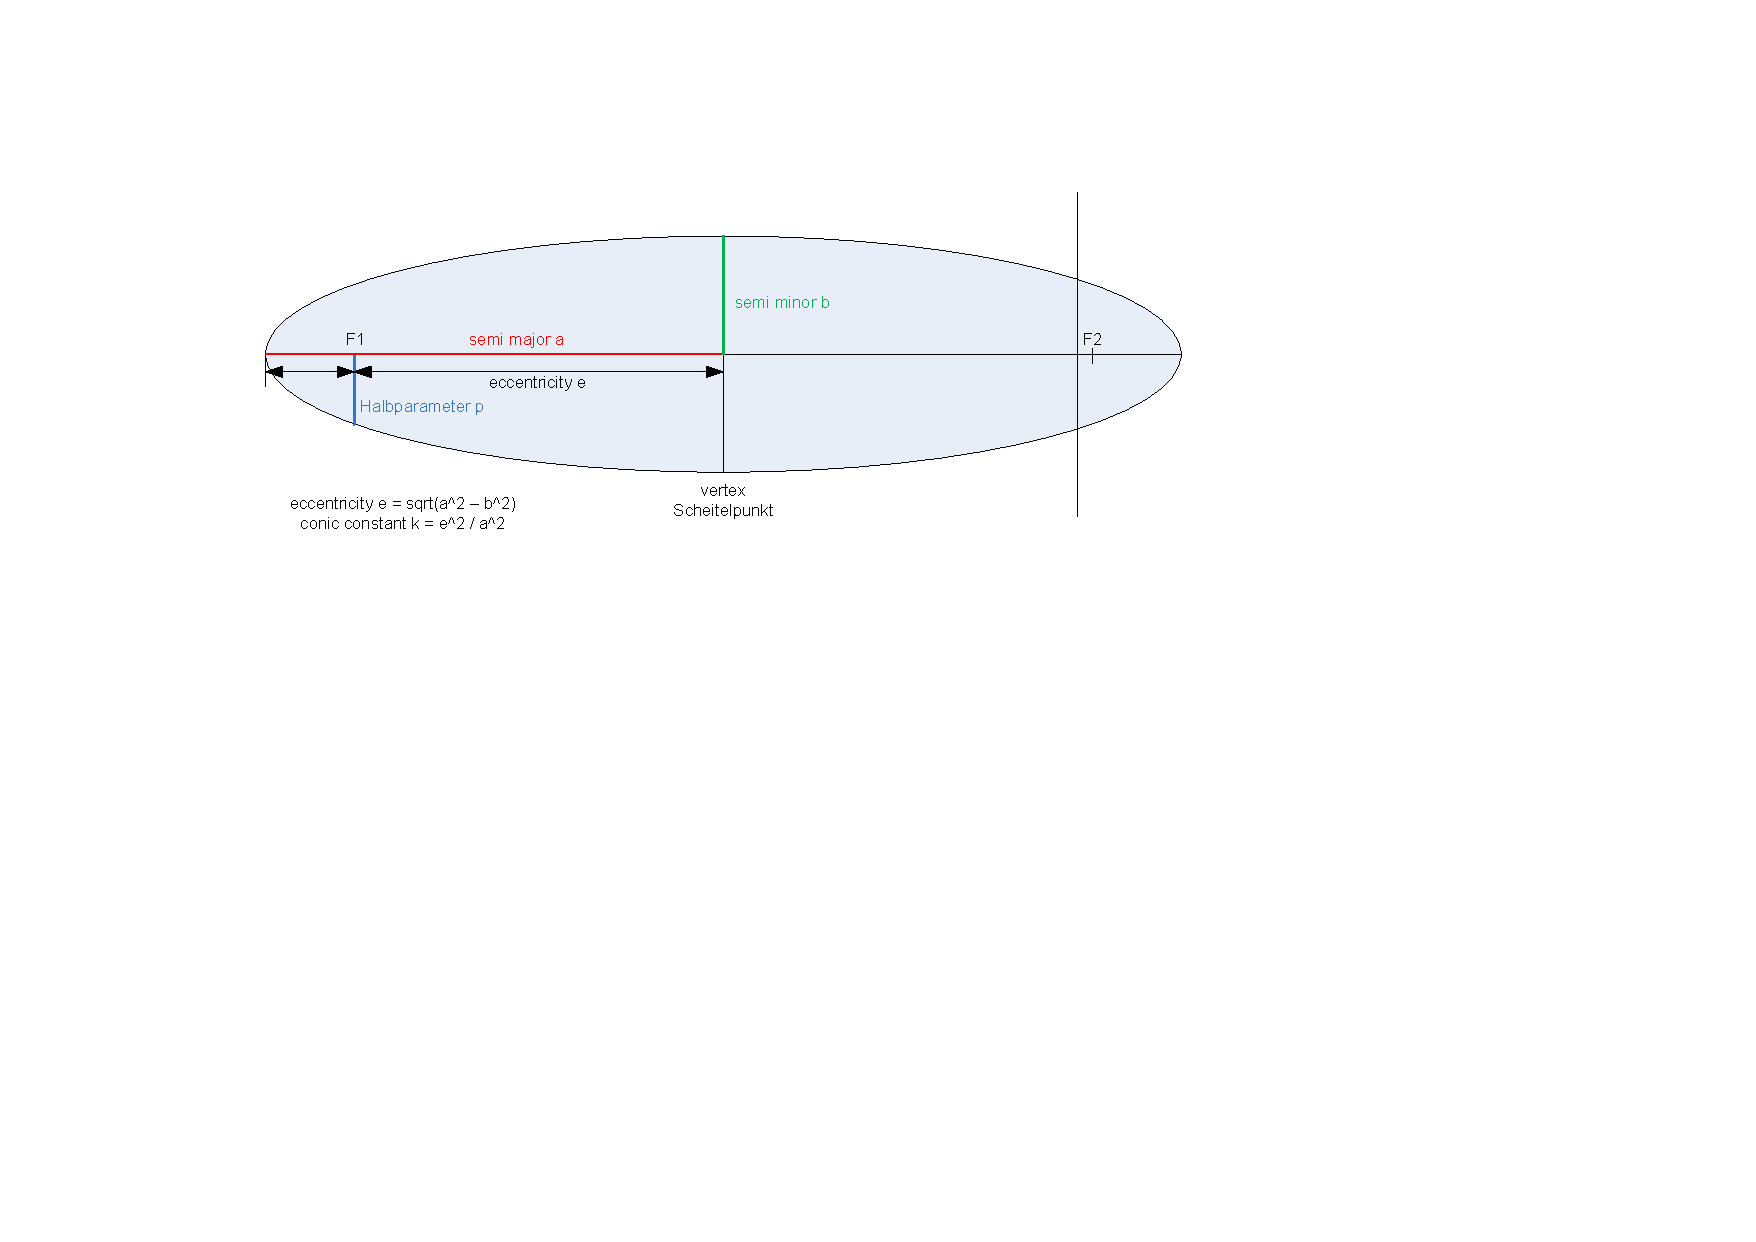
\includegraphics[width=0.9\textwidth, clip=true, trim = 80 10 0 10]{images/visio/visio.pdf}  % trim lm bm rm tm (left, bottom, right, top)
	\caption{clip=true, trim = 60 10 0 10}
	\label{fig.SkizzeZugeschnitten}
\end{figure}




\subsection{Mehrere Bilder nebeneinander}\label{nebeneinander}
Dank Minipages können mehrere Bilder auch nebeneinander sein:

%Zwei Bilder nebeneinander http://latex.mschroeder.net/
\begin{figure}[H]
  \centering
  \begin{minipage}[b]{0.45\textwidth}
    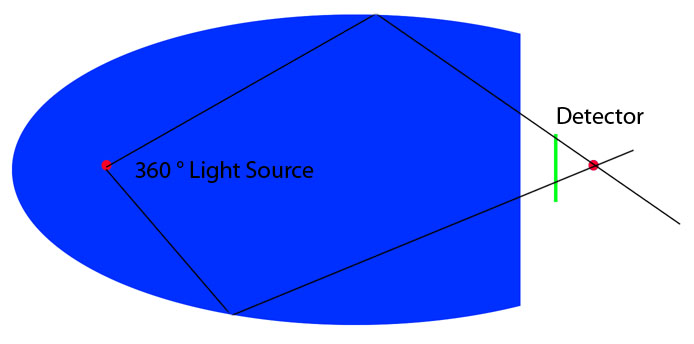
\includegraphics[scale=0.15]{images/photoshop/Skizze.jpg}
    \caption{Visir10b Detector}
    \label{Visir10bDetector} 
  \end{minipage} % Hier darf keine Leerzeile zwischen den beiden Minipages liegen!
  \begin{minipage}[b]{0.45\textwidth}
    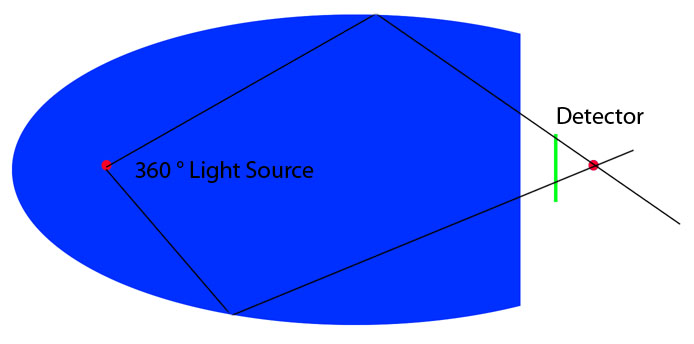
\includegraphics[scale=0.15]{images/photoshop/Skizze.jpg} 
    \caption{Visir10b Model}
    \label{Visir10bModel} 
  \end{minipage}
  \caption{Visir 10 mit optimiertem Reflektor}
  \label{fig.Visir10b}
\end{figure}


\section{Tabellen aufbauen}\label{tabelle}
Kleine Tabelle:

\begin{table}[ht] \centering
	\begin{tabular}{|p{3cm}|p{.5cm}|p{.5cm}|p{.5cm}|p{.5cm}|p{.5cm}|p{.5cm}|p{.5cm}|p{.5cm}|p{.5cm}|p{.5cm}|} \hline
		\rowcolor{gray} Modul & M01 & M02 & M03 & M04 & M05 & M06 & M07 & M08 & M09 & M10 \\
		\hline
		FPGA\_DATEN & & & & & X & X & & X & X & \\
		\hline
		IRQ & X & X & X & & X & & & & X & X \\
		\hline
		Nachbar Core & & & & X & & X & & X & & \\
		\hline
	\end{tabular}
	\caption{Port Schwierigkeiten der Funkmodule}
	\label{tab:portprobleme}
 \end{table}	

Die nachfolgende longtable kann sich über mehrere Seiten erstrecken.

\begin{longtable}{|p{1.1cm}|p{4cm}|p{4cm}|p{4cm}|} 
					\hline
					\rowcolor{gray} Typ & Variante A & Variante B & Variante C
					\\ \hline
					& \textbf{Vorteile:} 
							\begin{itemize}
								\item[+] hohe Spannungen
							\end{itemize}							
							\textbf{Nachteile:}
							\begin{itemize}
								\item[-] Grosse Abmessung
							\end{itemize}
					& 	\textbf{Vorteile:} 
							\begin{itemize}
								\item[+] einfache Montage
							\end{itemize}							
							\textbf{Nachteile:}
							\begin{itemize}
								\item[-] max. 2A Eingangsstrom
							\end{itemize}
					&	\textbf{Vorteile:} 
							\begin{itemize}
								\item[+] hoher Strom
							\end{itemize}							
							\textbf{Nachteile:}
							\begin{itemize}
								\item[-] max. 12 V Eingangsspannung
							\end{itemize}\\ \hline
						Zeit & 2 h & 5 h & 3 h \\ \hline
						Preis	& 520 CHF/Stück & 800 CHF/Stück &	360 CHF/Stück\\ \hline
				\caption{Morphologischer Kasten für die Speisung}
				\label{tab:morphkasten}
			\end{longtable}	

Diese Art von Tabelle erstreckt sich immer auf der ganzen Seitenlänge:

\begin{tabularx}{\textwidth}{XXl}
  Salat & Schnecke & Igel\\
  Montag & Hier ist ein langes Wort & Dienstag
\end{tabularx}



\section{Code Listings aufbauen}\label{listing}

\begin{lstlisting}[
    language=C++,
    caption={Test Kommandozeilen Ausgabe},
    label={list.Testoutput}
]
/********************************************************/
/* Name        : M07Setup                               */
/* Description : EM9201 init for adress and pck         */
/* Input       : targetadr (DevAdr_M00 - DevAdr_M39)    */
/*               drate (Drate_M00 - Drate_M39)          */
/* Ouput       : -0x01 -> Setup OK                      */
/*               -0x5E -> Setup Error Channel write     */
/*               -0x6E -> Setup Error power write       */
/*               -0x7E -> Error in Device Address       */
/*               -0x8E -> Error in Peer Address         */
/********************************************************/
\end{lstlisting}

Formula $e = \sqrt{a{^2} - b^{2}}$


Diese Textstelle ist sehr interessant.\label{interessant}\\
Hier wird auf die Textstelle~\ref{interessant} verwiesen, die sich auf der Seite~\pageref{interessant} befindet.


% nogo:
% \ref{src:miktex} (\nameref{src:miktex})



\section{Citation nach IEEE}\label{citation}

Das ist ein \cite{robotvision} Verweis aufs Literaturverzeichnis. Ein anderes Beispiel ist das hier \cite{randompatterns}.





Das ist eine Aufzählung:
\begin{itemize} %
	\item Erste Zeile
	\item Zweite Zeile
	\item Dritte Zeile
\end{itemize}


\begin{enumerate}
\item erstens
\item zweitens
\end{enumerate}

%https://parma.zhaw.ch/svn/zhw_latex/
%gmanstyle nötig unter start od begin einbinden


Das ist eine verschachtelte Aufzählung:
\begin{description}
		\item [Register Performance] Alle Signale die das FPGA nicht verlassen, also von FF zu FF weitergeleitet werden. Daraus ergibt sich die maximale Taktfrequenz F\textsubscript{MAX}.

		\item [Externes Timing] FPGA Ein- und Ausgänge
		\begin{itemize}
			\item Ausgänge = Von FF's durch Logik zu Ausgängen (t\textsubscript{CO})
			\item Eingänge = Von Eingängen durch Logik zu FF's (t\textsubscript{SU}, t\textsubscript{H})
			\item Durchgänge = kombinatorische Pfade durch das FPGA (t\textsubscript{PD})
		\end{itemize}
\end{description}
 % Für das Schlussdokument auskommentieren

%%%%%%%%%%%%%%%%%%%%%%%%%%%%%%%%%%%%%%%%%%%%%%%%%%%%%%%%%%%%%%%%%
%  _____   ____  _____                                          %
% |_   _| /  __||  __ \    Institute of Computitional Physics   %
%   | |  |  /   | |__) |   Zuercher Hochschule Winterthur       %
%   | |  | (    |  ___/    (University of Applied Sciences)     %
%  _| |_ |  \__ | |        8401 Winterthur, Switzerland         %
% |_____| \____||_|                                             %
%%%%%%%%%%%%%%%%%%%%%%%%%%%%%%%%%%%%%%%%%%%%%%%%%%%%%%%%%%%%%%%%%
%
% Project     : LaTeX doc Vorlage für Windows ProTeXt mit TexMakerX
% Title       : 
% File        : grundlagen.tex Rev. 00
% Date        : 7.5.12
% Author      : Remo Ritzmann
% Feedback bitte an Email: remo.ritzmann@pfunzle.ch
%
%%%%%%%%%%%%%%%%%%%%%%%%%%%%%%%%%%%%%%%%%%%%%%%%%%%%%%%%%%%%%%%%%

\chapter{(Theoretische Grundlagen)}\label{chap.grundlagen}
 % (2. Theoretische Grundlagen)
%%%%%%%%%%%%%%%%%%%%%%%%%%%%%%%%%%%%%%%%%%%%%%%%%%%%%%%%%%%%%%%%%
%  _____   ____  _____                                          %
% |_   _| /  __||  __ \    Institute of Computitional Physics   %
%   | |  |  /   | |__) |   Zuercher Hochschule Winterthur       %
%   | |  | (    |  ___/    (University of Applied Sciences)     %
%  _| |_ |  \__ | |        8401 Winterthur, Switzerland         %
% |_____| \____||_|                                             %
%%%%%%%%%%%%%%%%%%%%%%%%%%%%%%%%%%%%%%%%%%%%%%%%%%%%%%%%%%%%%%%%%
%
% Project     : LaTeX doc Vorlage für Windows ProTeXt mit TexMakerX
% Title       : 
% File        : vorgehen.tex Rev. 00
% Date        : 7.5.12
% Author      : Remo Ritzmann
% Feedback bitte an Email: remo.ritzmann@pfunzle.ch
%
%%%%%%%%%%%%%%%%%%%%%%%%%%%%%%%%%%%%%%%%%%%%%%%%%%%%%%%%%%%%%%%%%

\chapter{Vorgehen / Methoden}\label{chap.vorgehen}


\begin{itemize}
\item (Beschreibt die Grundüberlegungen der realisierten Lösung (Konstruktion/Entwurf) und die Realisierung als Simulation, als Prototyp oder als Software-Komponente)
\item (Definiert Messgrössen, beschreibt Mess- oder Versuchsaufbau, beschreibt und dokumentiert Durchführung der Messungen/Versuche)
\item (Experimente)
\item (Lösungsweg)
\item (Modell)
\item (Tests und Validierung)
\item (Theoretische Herleitung der Lösung)
\end{itemize}



\section{(Verwendete Software)}\label{software}
Für die vorliegende Arbeit wurden die unten aufgeführten Programme eingesetzt.

\subsection*{Arbeitsumgebung}\label{wintool}
\begin{itemize}
	\item Microsoft Windows 8 developer preview
\end{itemize}

\subsection*{Virtual Machine}\label{vm}
\begin{itemize}
	\item Oracle VM VirtualBox, Version 3.2.10
\end{itemize}

\subsection*{CAD Catia}\label{catia}
\begin{itemize}
	\item CATIA, Version 5.19 (in VirtualBox)
\end{itemize}

\subsection*{Dokumentation}\label{dokutools}
\begin{itemize}
	\item proTeXt mit TexMakerX 2.1 (SVN 1774), \href{http://www.latex-project.org/ftp.html}{latex-project.org}
	\item Microsoft Visio 2007
	\item Adobe Acrobat 8 Professional 8.1.6
\end{itemize}
 % Vorgehen / Methoden
%%%%%%%%%%%%%%%%%%%%%%%%%%%%%%%%%%%%%%%%%%%%%%%%%%%%%%%%%%%%%%%%%
%  _____   ____  _____                                          %
% |_   _| /  __||  __ \    Institute of Computitional Physics   %
%   | |  |  /   | |__) |   Zuercher Hochschule Winterthur       %
%   | |  | (    |  ___/    (University of Applied Sciences)     %
%  _| |_ |  \__ | |        8401 Winterthur, Switzerland         %
% |_____| \____||_|                                             %
%%%%%%%%%%%%%%%%%%%%%%%%%%%%%%%%%%%%%%%%%%%%%%%%%%%%%%%%%%%%%%%%%
%
% Project     : LaTeX doc Vorlage für Windows ProTeXt mit TexMakerX
% Title       : 
% File        : resultate.tex Rev. 00
% Date        : 23.4.12
% Author      : Remo Ritzmann
% Feedback bitte an Email: remo.ritzmann@pfunzle.ch
%
%%%%%%%%%%%%%%%%%%%%%%%%%%%%%%%%%%%%%%%%%%%%%%%%%%%%%%%%%%%%%%%%%

\chapter{Resultate}\label{chap.resultate} 

\begin{itemize}
\item (Zusammenfassung der Resultate)
\end{itemize}


\end{document}
